%%% Title presen22103
\documentclass[landscape,10pt]{ujarticle}
\special{papersize=\the\paperwidth,\the\paperheight}
\usepackage{ketpic,ketlayer}
\usepackage{ketslide}
\usepackage{amsmath,amssymb}
\usepackage{bm,enumerate}
\usepackage[dvipdfmx]{graphicx}
\usepackage{color}
\definecolor{slidecolora}{cmyk}{0.98,0.13,0,0.43}
\definecolor{slidecolorb}{cmyk}{0.2,0,0,0}
\definecolor{slidecolorc}{cmyk}{0.2,0,0,0}
\definecolor{slidecolord}{cmyk}{0.2,0,0,0}
\definecolor{slidecolore}{cmyk}{0,0,0,0.5}
\definecolor{slidecolorf}{cmyk}{0,0,0,0.5}
\definecolor{slidecolori}{cmyk}{0.98,0.13,0,0.43}
\def\setthin#1{\def\thin{#1}}
\setthin{0}
\newcommand{\slidepage}[1][s]{%
\setcounter{ketpicctra}{18}%
\if#1m \setcounter{ketpicctra}{1}\fi
\hypersetup{linkcolor=black}%

\begin{layer}{118}{0}
\putnotee{122}{-\theketpicctra.05}{\small\thepage/\pageref{pageend}}
\end{layer}\hypersetup{linkcolor=blue}

}
\usepackage{emath}
\usepackage{emathEy}
\usepackage{emathMw}
\usepackage{pict2e}
\usepackage{ketlayermorewith2e}
\usepackage[dvipdfmx,colorlinks=true,linkcolor=blue,filecolor=blue]{hyperref}
\newcommand{\hiduke}{0418}
\newcommand{\hako}[2][1]{\fbox{\raisebox{#1mm}{\mbox{}}\raisebox{-#1mm}{\mbox{}}\,\phantom{#2}\,}}
\newcommand{\hakoa}[2][1]{\fbox{\raisebox{#1mm}{\mbox{}}\raisebox{-#1mm}{\mbox{}}\,#2\,}}
\newcommand{\hakom}[2][1]{\hako[#1]{$#2$}}
\newcommand{\hakoma}[2][1]{\hakoa[#1]{$#2$}}
\def\rad{\;\mathrm{rad}}
\def\deg#1{#1^{\circ}}
\newcommand{\sbunsuu}[2]{\scalebox{0.6}{$\bunsuu{#1}{#2}$}}
\def\pow{$\hspace{-1.5mm}^\hspace{-1mm}$}
\def\dlim{\displaystyle\lim}
\newcommand{\brd}[2][1]{\scalebox{#1}{\color{red}\fbox{\color{black}$#2$}}}
\newcommand\down[1][0.5zw]{\vspace{#1}\\}

\setmargin{25}{145}{15}{100}

\ketslideinit

\pagestyle{empty}

\begin{document}

\begin{layer}{120}{0}
\putnotese{0}{0}{{\Large\bf
\color[cmyk]{1,1,0,0}

\begin{layer}{120}{0}
{\Huge \putnotes{60}{20}{三角関数の性質}}
\putnotes{60}{70}{2022.05.16}
\end{layer}

}
}
\end{layer}

\def\mainslidetitley{22}
\def\ketcletter{slidecolora}
\def\ketcbox{slidecolorb}
\def\ketdbox{slidecolorc}
\def\ketcframe{slidecolord}
\def\ketcshadow{slidecolore}
\def\ketdshadow{slidecolorf}
\def\slidetitlex{6}
\def\slidetitlesize{1.3}
\def\mketcletter{slidecolori}
\def\mketcbox{yellow}
\def\mketdbox{yellow}
\def\mketcframe{yellow}
\def\mslidetitlex{62}
\def\mslidetitlesize{2}

\color{black}
\Large\bf\boldmath
\addtocounter{page}{-1}

\def\MARU{}
\renewcommand{\MARU}[1]{{\ooalign{\hfil$#1$\/\hfil\crcr\raise.167ex\hbox{\mathhexbox20D}}}}
\renewcommand{\slidepage}[1][s]{%
\setcounter{ketpicctra}{18}%
\if#1m \setcounter{ketpicctra}{1}\fi
\hypersetup{linkcolor=black}%
\begin{layer}{118}{0}
\putnotee{115}{-\theketpicctra.05}{\small\hiduke-\thepage/\pageref{pageend}}
\end{layer}\hypersetup{linkcolor=blue}
}
\newcounter{ban}
\setcounter{ban}{1}
\newcommand{\monban}[1][\hiduke]{%
#1-\theban\ %
\addtocounter{ban}{1}%
}
\newcommand{\monbannoadd}[1][\hiduke]{%
#1-\theban\ %
}
\newcommand{\addban}{%
\addtocounter{ban}{1}%%210614
}
\newcounter{edawidth}
\newcounter{edactr}
\newcommand{\seteda}[1]{
\setcounter{edawidth}{#1}
\setcounter{edactr}{1}
}
\newcommand{\eda}[2][\theedawidth ]{%
\noindent\Ltab{#1 mm}{[\theedactr]\ #2}%
\addtocounter{edactr}{1}%
}
%%%%%%%%%%%%

%%%%%%%%%%%%%%%%%%%%

\mainslide{2次関数と方程式(復習+)}


\slidepage[m]
%%%%%%%%%%%%

%%%%%%%%%%%%%%%%%%%%

\newslide{2次関数のグラフ}

\vspace*{18mm}

\slidepage

\begin{layer}{120}{0}
\putnotese{90}{0}{\scalebox{0.7}{%%% /polytech22.git/103-0425/presen/fig/presen22103-1.2.tex 
%%% Generator=presen22103.cdy 
{\unitlength=1cm%
\begin{picture}%
(6,7)(-2,-2)%
\linethickness{0.008in}%%
\Large\bf\boldmath%
\small%
\linethickness{0.016in}%%
\polyline(-2.00000,4.00000)(-1.88000,3.53440)(-1.76000,3.09760)(-1.64000,2.68960)%
(-1.52000,2.31040)(-1.40000,1.96000)(-1.28000,1.63840)(-1.16000,1.34560)(-1.04000,1.08160)%
(-0.92000,0.84640)(-0.80000,0.64000)(-0.68000,0.46240)(-0.56000,0.31360)(-0.44000,0.19360)%
(-0.32000,0.10240)(-0.20000,0.04000)(-0.08000,0.00640)(0.04000,0.00160)(0.16000,0.02560)%
(0.28000,0.07840)(0.40000,0.16000)(0.52000,0.27040)(0.64000,0.40960)(0.76000,0.57760)%
(0.88000,0.77440)(1.00000,1.00000)(1.12000,1.25440)(1.24000,1.53760)(1.36000,1.84960)%
(1.48000,2.19040)(1.60000,2.56000)(1.72000,2.95840)(1.84000,3.38560)(1.96000,3.84160)%
(2.08000,4.32640)(2.20000,4.84000)(2.23540,5.00000)%
%
\linethickness{0.008in}%%
\linethickness{0.016in}%%
\polyline(0.00079,5.00000)(0.04000,4.84160)(0.16000,4.38560)(0.28000,3.95840)(0.40000,3.56000)%
(0.52000,3.19040)(0.64000,2.84960)(0.76000,2.53760)(0.88000,2.25440)(1.00000,2.00000)%
(1.12000,1.77440)(1.24000,1.57760)(1.36000,1.40960)(1.48000,1.27040)(1.60000,1.16000)%
(1.72000,1.07840)(1.84000,1.02560)(1.96000,1.00160)(2.08000,1.00640)(2.20000,1.04000)%
(2.32000,1.10240)(2.44000,1.19360)(2.56000,1.31360)(2.68000,1.46240)(2.80000,1.64000)%
(2.92000,1.84640)(3.04000,2.08160)(3.16000,2.34560)(3.28000,2.63840)(3.40000,2.96000)%
(3.52000,3.31040)(3.64000,3.68960)(3.76000,4.09760)(3.88000,4.53440)(4.00000,5.00000)%
%
\linethickness{0.008in}%%
\polyline(2.00000,0.00000)(2.00000,0.09677)\polyline(2.00000,0.19355)(2.00000,0.29032)%
\polyline(2.00000,0.38710)(2.00000,0.48387)\polyline(2.00000,0.58065)(2.00000,0.67742)%
\polyline(2.00000,0.77419)(2.00000,0.87097)\polyline(2.00000,0.96774)(2.00000,1.00000)(1.93548,1.00000)%
\polyline(1.83871,1.00000)(1.74194,1.00000)\polyline(1.64516,1.00000)(1.54839,1.00000)%
\polyline(1.45161,1.00000)(1.35484,1.00000)\polyline(1.25806,1.00000)(1.16129,1.00000)%
\polyline(1.06452,1.00000)(0.96774,1.00000)\polyline(0.87097,1.00000)(0.77419,1.00000)%
\polyline(0.67742,1.00000)(0.58065,1.00000)\polyline(0.48387,1.00000)(0.38710,1.00000)%
\polyline(0.29032,1.00000)(0.19355,1.00000)\polyline(0.09677,1.00000)(0.00000,1.00000)%
%
%
\polyline(2.00000,0.05000)(2.00000,-0.05000)%
%
\settowidth{\Width}{$b$}\setlength{\Width}{-0.5\Width}%
\settoheight{\Height}{$b$}\settodepth{\Depth}{$b$}\setlength{\Height}{-\Height}%
\put(2.0000000,-0.1000000){\hspace*{\Width}\raisebox{\Height}{$b$}}%
%
\polyline(0.05000,1.00000)(-0.05000,1.00000)%
%
\settowidth{\Width}{$c$}\setlength{\Width}{-1\Width}%
\settoheight{\Height}{$c$}\settodepth{\Depth}{$c$}\setlength{\Height}{-0.5\Height}\setlength{\Depth}{0.5\Depth}\addtolength{\Height}{\Depth}%
\put(-0.1000000,1.0000000){\hspace*{\Width}\raisebox{\Height}{$c$}}%
%
\polyline(-2.00000,0.00000)(4.00000,0.00000)%
%
\polyline(0.00000,-2.00000)(0.00000,5.00000)%
%
\settowidth{\Width}{$x$}\setlength{\Width}{0\Width}%
\settoheight{\Height}{$x$}\settodepth{\Depth}{$x$}\setlength{\Height}{-0.5\Height}\setlength{\Depth}{0.5\Depth}\addtolength{\Height}{\Depth}%
\put(4.0500000,0.0000000){\hspace*{\Width}\raisebox{\Height}{$x$}}%
%
\settowidth{\Width}{$y$}\setlength{\Width}{-0.5\Width}%
\settoheight{\Height}{$y$}\settodepth{\Depth}{$y$}\setlength{\Height}{\Depth}%
\put(0.0000000,5.0500000){\hspace*{\Width}\raisebox{\Height}{$y$}}%
%
\settowidth{\Width}{O}\setlength{\Width}{-1\Width}%
\settoheight{\Height}{O}\settodepth{\Depth}{O}\setlength{\Height}{-\Height}%
\put(-0.0500000,-0.0500000){\hspace*{\Width}\raisebox{\Height}{O}}%
%
\end{picture}}%}}
\end{layer}

\begin{enumerate}[(1)]
\item
$y=a(x-b)^2+c$\\
 ・$y=ax^2$のグラフと形は同じ\\
 ・$x$方向に$b$,$y$方向に$c$平行移動\\
 ・頂点は $(b,\ c)$\vspace{-2mm}
\item
$y=ax^2+bx+c$\\
 ・(1)の形に変形(平方完成)\\
 ・例)$y=x^2+4x+1$\\
    $\phantom{y}=(x^2+4x+4)-4+1=(x+2)^2-3$\\
    頂点は $(-2,-3)$
\end{enumerate}

\newslide{2次方程式の解}

\vspace*{18mm}

\slidepage

\begin{layer}{120}{0}
\putnotese{90}{0}{\scalebox{0.7}{%%% /polytech22.git/103-0425/presen/fig/presen22103-2.tex 
%%% Generator=presen22103.cdy 
{\unitlength=1cm%
\begin{picture}%
(6,7)(-3,-3)%
\linethickness{0.008in}%%
\Large\bf\boldmath%
\small%
\linethickness{0.016in}%%
\polyline(-2.21150,4.00000)(-2.16000,3.74560)(-2.04000,3.18160)(-1.92000,2.64640)%
(-1.80000,2.14000)(-1.68000,1.66240)(-1.56000,1.21360)(-1.44000,0.79360)(-1.32000,0.40240)%
(-1.20000,0.04000)(-1.08000,-0.29360)(-0.96000,-0.59840)(-0.84000,-0.87440)(-0.72000,-1.12160)%
(-0.60000,-1.34000)(-0.48000,-1.52960)(-0.36000,-1.69040)(-0.24000,-1.82240)(-0.12000,-1.92560)%
(0.00000,-2.00000)(0.12000,-2.04560)(0.24000,-2.06240)(0.36000,-2.05040)(0.48000,-2.00960)%
(0.60000,-1.94000)(0.72000,-1.84160)(0.84000,-1.71440)(0.96000,-1.55840)(1.08000,-1.37360)%
(1.20000,-1.16000)(1.32000,-0.91760)(1.44000,-0.64640)(1.56000,-0.34640)(1.68000,-0.01760)%
(1.80000,0.34000)(1.92000,0.72640)(2.04000,1.14160)(2.16000,1.58560)(2.28000,2.05840)%
(2.40000,2.56000)(2.52000,3.09040)(2.64000,3.64960)(2.71151,4.00000)%
%
\linethickness{0.008in}%%
\settowidth{\Width}{$\alpha$}\setlength{\Width}{-1\Width}%
\settoheight{\Height}{$\alpha$}\settodepth{\Depth}{$\alpha$}\setlength{\Height}{-\Height}%
\put(-1.2900000,-0.1000000){\hspace*{\Width}\raisebox{\Height}{$\alpha$}}%
%
\settowidth{\Width}{$\beta$}\setlength{\Width}{0\Width}%
\settoheight{\Height}{$\beta$}\settodepth{\Depth}{$\beta$}\setlength{\Height}{-\Height}%
\put(1.7900000,-0.1000000){\hspace*{\Width}\raisebox{\Height}{$\beta$}}%
%
\polyline(-3.00000,0.00000)(3.00000,0.00000)%
%
\polyline(0.00000,-3.00000)(0.00000,4.00000)%
%
\settowidth{\Width}{$x$}\setlength{\Width}{0\Width}%
\settoheight{\Height}{$x$}\settodepth{\Depth}{$x$}\setlength{\Height}{-0.5\Height}\setlength{\Depth}{0.5\Depth}\addtolength{\Height}{\Depth}%
\put(3.0500000,0.0000000){\hspace*{\Width}\raisebox{\Height}{$x$}}%
%
\settowidth{\Width}{$y$}\setlength{\Width}{-0.5\Width}%
\settoheight{\Height}{$y$}\settodepth{\Depth}{$y$}\setlength{\Height}{\Depth}%
\put(0.0000000,4.0500000){\hspace*{\Width}\raisebox{\Height}{$y$}}%
%
\settowidth{\Width}{O}\setlength{\Width}{-1\Width}%
\settoheight{\Height}{O}\settodepth{\Depth}{O}\setlength{\Height}{-\Height}%
\put(-0.0500000,-0.0500000){\hspace*{\Width}\raisebox{\Height}{O}}%
%
\end{picture}}%}}
\end{layer}

\begin{itemize}
\item
方程式$ax^2+bx+c=0$の解は\\
 $y=ax^2+bx+c$のグラフと\\
 $x$軸との交点の$x$座標
\item
[課題]\monbannoadd グラフをかき,\\
\phantom{\monban}方程式の解を求めよ\seteda{110}\\
\eda{$y=x^2-2x-3,\ x^2-2x-3=0$}\\
\eda{$y=2x^2+7x-4,\ 2x^2+7x-4=0$}
\end{itemize}

\newslide{解の公式1}

\vspace*{18mm}

\slidepage
\begin{itemize}
\item
$x^2+2ax+b=0$
\\$(x+a)^2-a^2+b=0$
\\$(x+a)^2=a^2-b$
\\$x+a=\pm \sqrt{a^2-b}$
\vspace{2mm}\\よって \fbox{\color{red}$x=-a\pm \sqrt{a^2-b}$}
\end{itemize}

\newslide{解の公式2}

\vspace*{18mm}

\slidepage
\begin{itemize}
\item
2次方程式$ax^2+bx+c=0$の解\vspace{1mm}\\
\hspace*{3zw}\fbox{$x=\bunsuu{-b\pm\sqrt{b^2-4ac}}{2a}$}\vspace{-2mm}
\item
[]例)$2x^2-5x+1=0$\\
\hspace*{3zw}$x=\bunsuu{5\pm \sqrt{5^2-4\cdot 2\cdot1}}{2\cdot 2}$
$=\bunsuu{5\pm \sqrt{17}}{4}$\vspace{-2mm}
\item
[課題] \monban 次の2次方程式を解け.\hfill Text P.74\seteda{55}\\
\eda{$2x^2+2x-3=0$}\eda{$3x^2+5x+1=0$}\\
\eda{$2x^2+x-2=0$}\eda{$x^2+3x+1=0$}
\end{itemize}

\mainslide{三角比}


\slidepage[m]
%%%%%%%%%%%%

%%%%%%%%%%%%%%%%%%%%

\newslide{三平方の定理}

\vspace*{18mm}

\slidepage

\begin{layer}{120}{0}
\putnotene{90}{35}{%%% /Users/takatoosetsuo/Dropbox/2021polytech/103/fig/presen10310303.tex 
%%% Generator=presen103.cdy 
{\unitlength=7mm%
\begin{picture}%
(4,3.5)(0,-0.5)%
\special{pn 8}%
%
\Large\bf\boldmath%
\small%
\normalsize%
\special{pn 16}%
\special{pa   933  -620}\special{pa     0    -0}\special{pa   933    -0}\special{pa   933  -620}%
\special{fp}%
\special{pn 8}%
\special{pn 4}%
\special{pa    -0    -0}\special{pa     8     3}\special{pa    16     7}\special{pa    24    10}%
\special{pa    33    13}\special{pa    41    16}\special{pa    49    19}\special{pa    57    22}%
\special{pa    65    25}\special{pa    74    28}\special{pa    82    31}\special{pa    90    33}%
\special{pa    99    36}\special{pa   107    39}\special{pa   115    41}\special{pa   124    44}%
\special{pa   132    46}\special{pa   141    49}\special{pa   149    51}\special{pa   157    53}%
\special{pa   166    55}\special{pa   174    58}\special{pa   183    60}\special{pa   191    62}%
\special{pa   200    64}\special{pa   209    66}\special{pa   217    67}\special{pa   226    69}%
\special{pa   234    71}\special{pa   243    73}\special{pa   251    74}\special{pa   260    76}%
\special{pa   269    77}\special{pa   277    78}\special{pa   286    80}\special{pa   295    81}%
\special{pa   303    82}\special{pa   312    83}\special{pa   321    85}\special{pa   329    86}%
\special{pa   338    87}\special{pa   347    87}\special{pa   356    88}\special{pa   364    89}%
\special{pa   373    90}\special{pa   382    90}\special{pa   390    91}\special{pa   399    91}%
\special{pa   408    92}\special{pa   417    92}\special{pa   425    93}%
\special{fp}%
\special{pa   508    93}\special{pa   517    92}\special{pa   526    92}\special{pa   534    91}%
\special{pa   543    91}\special{pa   552    90}\special{pa   561    90}\special{pa   569    89}%
\special{pa   578    88}\special{pa   587    87}\special{pa   595    87}\special{pa   604    86}%
\special{pa   613    85}\special{pa   621    83}\special{pa   630    82}\special{pa   639    81}%
\special{pa   647    80}\special{pa   656    78}\special{pa   665    77}\special{pa   673    76}%
\special{pa   682    74}\special{pa   691    73}\special{pa   699    71}\special{pa   708    69}%
\special{pa   716    67}\special{pa   725    66}\special{pa   734    64}\special{pa   742    62}%
\special{pa   751    60}\special{pa   759    58}\special{pa   768    55}\special{pa   776    53}%
\special{pa   784    51}\special{pa   793    49}\special{pa   801    46}\special{pa   810    44}%
\special{pa   818    41}\special{pa   827    39}\special{pa   835    36}\special{pa   843    33}%
\special{pa   852    31}\special{pa   860    28}\special{pa   868    25}\special{pa   876    22}%
\special{pa   885    19}\special{pa   893    16}\special{pa   901    13}\special{pa   909    10}%
\special{pa   917     7}\special{pa   925     3}\special{pa   933     0}%
\special{fp}%
\special{pn 8}%
\settowidth{\Width}{$a$}\setlength{\Width}{-0.5\Width}%
\settoheight{\Height}{$a$}\settodepth{\Depth}{$a$}\setlength{\Height}{-0.5\Height}\setlength{\Depth}{0.5\Depth}\addtolength{\Height}{\Depth}%
\put(1.6900000,-0.3400000){\hspace*{\Width}\raisebox{\Height}{$a$}}%
%
\special{pn 4}%
\special{pa   933     0}\special{pa   936    -5}\special{pa   938   -10}\special{pa   940   -15}%
\special{pa   942   -21}\special{pa   944   -26}\special{pa   946   -31}\special{pa   948   -36}%
\special{pa   949   -41}\special{pa   951   -47}\special{pa   953   -52}\special{pa   955   -57}%
\special{pa   956   -62}\special{pa   958   -68}\special{pa   960   -73}\special{pa   961   -78}%
\special{pa   963   -83}\special{pa   965   -89}\special{pa   966   -94}\special{pa   968   -99}%
\special{pa   969  -105}\special{pa   970  -110}\special{pa   972  -116}\special{pa   973  -121}%
\special{pa   974  -126}\special{pa   976  -132}\special{pa   977  -137}\special{pa   978  -143}%
\special{pa   979  -148}\special{pa   980  -153}\special{pa   981  -159}\special{pa   982  -164}%
\special{pa   983  -170}\special{pa   984  -175}\special{pa   985  -181}\special{pa   986  -186}%
\special{pa   987  -192}\special{pa   988  -197}\special{pa   988  -203}\special{pa   989  -208}%
\special{pa   990  -214}\special{pa   990  -219}\special{pa   991  -225}\special{pa   992  -230}%
\special{pa   992  -236}\special{pa   993  -241}\special{pa   993  -247}\special{pa   993  -252}%
\special{pa   994  -258}\special{pa   994  -263}\special{pa   994  -269}%
\special{fp}%
\special{pa   994  -351}\special{pa   994  -357}\special{pa   994  -362}\special{pa   993  -368}%
\special{pa   993  -373}\special{pa   993  -379}\special{pa   992  -384}\special{pa   992  -390}%
\special{pa   991  -395}\special{pa   990  -401}\special{pa   990  -406}\special{pa   989  -412}%
\special{pa   988  -417}\special{pa   988  -423}\special{pa   987  -428}\special{pa   986  -434}%
\special{pa   985  -439}\special{pa   984  -445}\special{pa   983  -450}\special{pa   982  -456}%
\special{pa   981  -461}\special{pa   980  -467}\special{pa   979  -472}\special{pa   978  -477}%
\special{pa   977  -483}\special{pa   976  -488}\special{pa   974  -494}\special{pa   973  -499}%
\special{pa   972  -504}\special{pa   970  -510}\special{pa   969  -515}\special{pa   968  -521}%
\special{pa   966  -526}\special{pa   965  -531}\special{pa   963  -537}\special{pa   961  -542}%
\special{pa   960  -547}\special{pa   958  -552}\special{pa   956  -558}\special{pa   955  -563}%
\special{pa   953  -568}\special{pa   951  -573}\special{pa   949  -579}\special{pa   948  -584}%
\special{pa   946  -589}\special{pa   944  -594}\special{pa   942  -599}\special{pa   940  -605}%
\special{pa   938  -610}\special{pa   936  -615}\special{pa   933  -620}%
\special{fp}%
\special{pn 8}%
\settowidth{\Width}{$b$}\setlength{\Width}{-0.5\Width}%
\settoheight{\Height}{$b$}\settodepth{\Depth}{$b$}\setlength{\Height}{-0.5\Height}\setlength{\Depth}{0.5\Depth}\addtolength{\Height}{\Depth}%
\put(3.6100000,1.1200000){\hspace*{\Width}\raisebox{\Height}{$b$}}%
%
\special{pn 4}%
\special{pa   933  -620}\special{pa   923  -618}\special{pa   913  -616}\special{pa   902  -614}%
\special{pa   892  -611}\special{pa   881  -609}\special{pa   871  -606}\special{pa   861  -604}%
\special{pa   850  -601}\special{pa   840  -599}\special{pa   830  -596}\special{pa   819  -593}%
\special{pa   809  -590}\special{pa   799  -587}\special{pa   788  -584}\special{pa   778  -581}%
\special{pa   768  -578}\special{pa   758  -574}\special{pa   748  -571}\special{pa   738  -568}%
\special{pa   728  -564}\special{pa   718  -561}\special{pa   708  -557}\special{pa   697  -553}%
\special{pa   688  -549}\special{pa   678  -546}\special{pa   668  -542}\special{pa   658  -538}%
\special{pa   648  -534}\special{pa   638  -529}\special{pa   628  -525}\special{pa   618  -521}%
\special{pa   609  -516}\special{pa   599  -512}\special{pa   589  -507}\special{pa   580  -503}%
\special{pa   570  -498}\special{pa   561  -493}\special{pa   551  -489}\special{pa   542  -484}%
\special{pa   532  -479}\special{pa   523  -474}\special{pa   513  -469}\special{pa   504  -464}%
\special{pa   495  -458}\special{pa   485  -453}\special{pa   476  -448}\special{pa   467  -442}%
\special{pa   458  -437}\special{pa   449  -431}\special{pa   439  -426}%
\special{fp}%
\special{pa   371  -380}\special{pa   362  -374}\special{pa   353  -368}\special{pa   345  -361}%
\special{pa   336  -355}\special{pa   328  -348}\special{pa   319  -342}\special{pa   311  -335}%
\special{pa   302  -329}\special{pa   294  -322}\special{pa   286  -315}\special{pa   278  -308}%
\special{pa   269  -302}\special{pa   261  -295}\special{pa   253  -288}\special{pa   245  -281}%
\special{pa   237  -274}\special{pa   229  -266}\special{pa   221  -259}\special{pa   214  -252}%
\special{pa   206  -245}\special{pa   198  -237}\special{pa   190  -230}\special{pa   183  -222}%
\special{pa   175  -215}\special{pa   168  -207}\special{pa   160  -199}\special{pa   153  -192}%
\special{pa   146  -184}\special{pa   139  -176}\special{pa   131  -168}\special{pa   124  -160}%
\special{pa   117  -152}\special{pa   110  -144}\special{pa   103  -136}\special{pa    96  -128}%
\special{pa    89  -120}\special{pa    83  -111}\special{pa    76  -103}\special{pa    69   -95}%
\special{pa    63   -86}\special{pa    56   -78}\special{pa    50   -70}\special{pa    43   -61}%
\special{pa    37   -52}\special{pa    30   -44}\special{pa    24   -35}\special{pa    18   -26}%
\special{pa    12   -18}\special{pa     6    -9}\special{pa    -0     0}%
\special{fp}%
\special{pn 8}%
\settowidth{\Width}{$c$}\setlength{\Width}{-0.5\Width}%
\settoheight{\Height}{$c$}\settodepth{\Depth}{$c$}\setlength{\Height}{-0.5\Height}\setlength{\Depth}{0.5\Depth}\addtolength{\Height}{\Depth}%
\put(1.4700000,1.4600000){\hspace*{\Width}\raisebox{\Height}{$c$}}%
%
\special{pn 4}%
\special{pa   819  -544}\special{pa   822  -539}\special{pa   833  -526}\special{pa   846  -514}%
\special{pa   860  -504}\special{pa   875  -495}\special{pa   891  -489}\special{pa   908  -485}%
\special{pa   925  -482}\special{pa   933  -482}%
\special{fp}%
\special{pn 8}%
\settowidth{\Width}{$A$}\setlength{\Width}{-0.5\Width}%
\settoheight{\Height}{$A$}\settodepth{\Depth}{$A$}\setlength{\Height}{-0.5\Height}\setlength{\Depth}{0.5\Depth}\addtolength{\Height}{\Depth}%
\put(3.0200000,1.5600000){\hspace*{\Width}\raisebox{\Height}{$A$}}%
%
\special{pa   933   -69}\special{pa   865   -69}\special{pa   865    -0}%
\special{fp}%
\special{pa   138    -0}\special{pa   137   -17}\special{pa   133   -34}\special{pa   128   -51}%
\special{pa   121   -66}\special{pa   115   -76}%
\special{fp}%
\settowidth{\Width}{$B$}\setlength{\Width}{-0.5\Width}%
\settoheight{\Height}{$B$}\settodepth{\Depth}{$B$}\setlength{\Height}{-0.5\Height}\setlength{\Depth}{0.5\Depth}\addtolength{\Height}{\Depth}%
\put(0.7500000,0.2300000){\hspace*{\Width}\raisebox{\Height}{$B$}}%
%
\settowidth{\Width}{A}\setlength{\Width}{-0.5\Width}%
\settoheight{\Height}{A}\settodepth{\Depth}{A}\setlength{\Height}{\Depth}%
\put(3.3900000,2.3928571){\hspace*{\Width}\raisebox{\Height}{A}}%
%
\settowidth{\Width}{B}\setlength{\Width}{-1\Width}%
\settoheight{\Height}{B}\settodepth{\Depth}{B}\setlength{\Height}{-0.5\Height}\setlength{\Depth}{0.5\Depth}\addtolength{\Height}{\Depth}%
\put(-0.1428571,0.0000000){\hspace*{\Width}\raisebox{\Height}{B}}%
%
\settowidth{\Width}{C}\setlength{\Width}{0\Width}%
\settoheight{\Height}{C}\settodepth{\Depth}{C}\setlength{\Height}{-0.5\Height}\setlength{\Depth}{0.5\Depth}\addtolength{\Height}{\Depth}%
\put(3.5328571,0.0000000){\hspace*{\Width}\raisebox{\Height}{C}}%
%
\end{picture}}%}
\putnotene{10}{70}{%%% /Users/takatoosetsuo/Dropbox/2021polytech/103/fig/presen10310304a.tex 
%%% Generator=presen103.cdy 
{\unitlength=7mm%
\begin{picture}%
(4.5,4.5)(0,-0.5)%
\special{pn 8}%
%
\Large\bf\boldmath%
\small%
\normalsize%
\special{pn 16}%
\special{pa  1102  -827}\special{pa     0    -0}\special{pa  1102    -0}\special{pa  1102  -827}%
\special{fp}%
\special{pn 8}%
\special{pn 4}%
\special{pa    -0    -0}\special{pa    10     4}\special{pa    19     8}\special{pa    29    12}%
\special{pa    39    16}\special{pa    49    19}\special{pa    59    23}\special{pa    68    26}%
\special{pa    78    30}\special{pa    88    33}\special{pa    98    37}\special{pa   108    40}%
\special{pa   118    43}\special{pa   128    46}\special{pa   138    49}\special{pa   148    52}%
\special{pa   158    55}\special{pa   168    58}\special{pa   179    61}\special{pa   189    64}%
\special{pa   199    66}\special{pa   209    69}\special{pa   219    71}\special{pa   229    74}%
\special{pa   240    76}\special{pa   250    78}\special{pa   260    80}\special{pa   270    82}%
\special{pa   281    84}\special{pa   291    86}\special{pa   301    88}\special{pa   312    90}%
\special{pa   322    92}\special{pa   332    93}\special{pa   343    95}\special{pa   353    96}%
\special{pa   364    98}\special{pa   374    99}\special{pa   384   100}\special{pa   395   102}%
\special{pa   405   103}\special{pa   416   104}\special{pa   426   105}\special{pa   437   106}%
\special{pa   447   106}\special{pa   457   107}\special{pa   468   108}\special{pa   478   108}%
\special{pa   489   109}\special{pa   499   109}\special{pa   510   110}%
\special{fp}%
\special{pa   593   110}\special{pa   603   109}\special{pa   613   109}\special{pa   624   108}%
\special{pa   634   108}\special{pa   645   107}\special{pa   655   106}\special{pa   666   106}%
\special{pa   676   105}\special{pa   687   104}\special{pa   697   103}\special{pa   708   102}%
\special{pa   718   100}\special{pa   728    99}\special{pa   739    98}\special{pa   749    96}%
\special{pa   760    95}\special{pa   770    93}\special{pa   780    92}\special{pa   791    90}%
\special{pa   801    88}\special{pa   811    86}\special{pa   822    84}\special{pa   832    82}%
\special{pa   842    80}\special{pa   852    78}\special{pa   863    76}\special{pa   873    74}%
\special{pa   883    71}\special{pa   893    69}\special{pa   904    66}\special{pa   914    64}%
\special{pa   924    61}\special{pa   934    58}\special{pa   944    55}\special{pa   954    52}%
\special{pa   964    49}\special{pa   974    46}\special{pa   984    43}\special{pa   994    40}%
\special{pa  1004    37}\special{pa  1014    33}\special{pa  1024    30}\special{pa  1034    26}%
\special{pa  1044    23}\special{pa  1054    19}\special{pa  1063    16}\special{pa  1073    12}%
\special{pa  1083     8}\special{pa  1093     4}\special{pa  1102     0}%
\special{fp}%
\special{pn 8}%
\settowidth{\Width}{$4$}\setlength{\Width}{-0.5\Width}%
\settoheight{\Height}{$4$}\settodepth{\Depth}{$4$}\setlength{\Height}{-0.5\Height}\setlength{\Depth}{0.5\Depth}\addtolength{\Height}{\Depth}%
\put(2.0000000,-0.4000000){\hspace*{\Width}\raisebox{\Height}{$4$}}%
%
\special{pn 4}%
\special{pa  1102     0}\special{pa  1105    -7}\special{pa  1108   -14}\special{pa  1111   -21}%
\special{pa  1114   -28}\special{pa  1116   -36}\special{pa  1119   -43}\special{pa  1122   -50}%
\special{pa  1124   -57}\special{pa  1127   -64}\special{pa  1129   -72}\special{pa  1132   -79}%
\special{pa  1134   -86}\special{pa  1136   -94}\special{pa  1139  -101}\special{pa  1141  -108}%
\special{pa  1143  -116}\special{pa  1145  -123}\special{pa  1147  -130}\special{pa  1149  -138}%
\special{pa  1151  -145}\special{pa  1153  -153}\special{pa  1155  -160}\special{pa  1157  -167}%
\special{pa  1158  -175}\special{pa  1160  -182}\special{pa  1162  -190}\special{pa  1163  -197}%
\special{pa  1165  -205}\special{pa  1166  -212}\special{pa  1167  -220}\special{pa  1169  -227}%
\special{pa  1170  -235}\special{pa  1171  -243}\special{pa  1173  -250}\special{pa  1174  -258}%
\special{pa  1175  -265}\special{pa  1176  -273}\special{pa  1177  -280}\special{pa  1178  -288}%
\special{pa  1179  -296}\special{pa  1179  -303}\special{pa  1180  -311}\special{pa  1181  -319}%
\special{pa  1181  -326}\special{pa  1182  -334}\special{pa  1183  -341}\special{pa  1183  -349}%
\special{pa  1184  -357}\special{pa  1184  -364}\special{pa  1184  -372}%
\special{fp}%
\special{pa  1184  -455}\special{pa  1184  -462}\special{pa  1184  -470}\special{pa  1183  -478}%
\special{pa  1183  -485}\special{pa  1182  -493}\special{pa  1181  -501}\special{pa  1181  -508}%
\special{pa  1180  -516}\special{pa  1179  -523}\special{pa  1179  -531}\special{pa  1178  -539}%
\special{pa  1177  -546}\special{pa  1176  -554}\special{pa  1175  -561}\special{pa  1174  -569}%
\special{pa  1173  -577}\special{pa  1171  -584}\special{pa  1170  -592}\special{pa  1169  -599}%
\special{pa  1167  -607}\special{pa  1166  -614}\special{pa  1165  -622}\special{pa  1163  -629}%
\special{pa  1162  -637}\special{pa  1160  -644}\special{pa  1158  -652}\special{pa  1157  -659}%
\special{pa  1155  -667}\special{pa  1153  -674}\special{pa  1151  -682}\special{pa  1149  -689}%
\special{pa  1147  -696}\special{pa  1145  -704}\special{pa  1143  -711}\special{pa  1141  -719}%
\special{pa  1139  -726}\special{pa  1136  -733}\special{pa  1134  -741}\special{pa  1132  -748}%
\special{pa  1129  -755}\special{pa  1127  -762}\special{pa  1124  -770}\special{pa  1122  -777}%
\special{pa  1119  -784}\special{pa  1116  -791}\special{pa  1114  -798}\special{pa  1111  -805}%
\special{pa  1108  -813}\special{pa  1105  -820}\special{pa  1102  -827}%
\special{fp}%
\special{pn 8}%
\settowidth{\Width}{$b$}\setlength{\Width}{-0.5\Width}%
\settoheight{\Height}{$b$}\settodepth{\Depth}{$b$}\setlength{\Height}{-0.5\Height}\setlength{\Depth}{0.5\Depth}\addtolength{\Height}{\Depth}%
\put(4.3000000,1.5000000){\hspace*{\Width}\raisebox{\Height}{$b$}}%
%
\special{pn 4}%
\special{pa  1102  -827}\special{pa  1089  -823}\special{pa  1077  -820}\special{pa  1064  -817}%
\special{pa  1051  -813}\special{pa  1038  -809}\special{pa  1025  -805}\special{pa  1013  -801}%
\special{pa  1000  -797}\special{pa   987  -793}\special{pa   975  -789}\special{pa   962  -785}%
\special{pa   949  -781}\special{pa   937  -776}\special{pa   924  -772}\special{pa   912  -767}%
\special{pa   899  -762}\special{pa   887  -757}\special{pa   875  -752}\special{pa   862  -747}%
\special{pa   850  -742}\special{pa   838  -737}\special{pa   826  -732}\special{pa   813  -726}%
\special{pa   801  -721}\special{pa   789  -715}\special{pa   777  -710}\special{pa   765  -704}%
\special{pa   753  -698}\special{pa   741  -692}\special{pa   729  -686}\special{pa   717  -680}%
\special{pa   706  -674}\special{pa   694  -668}\special{pa   682  -661}\special{pa   671  -655}%
\special{pa   659  -648}\special{pa   647  -642}\special{pa   636  -635}\special{pa   624  -628}%
\special{pa   613  -621}\special{pa   602  -614}\special{pa   590  -607}\special{pa   579  -600}%
\special{pa   568  -593}\special{pa   557  -586}\special{pa   546  -578}\special{pa   535  -571}%
\special{pa   524  -563}\special{pa   513  -556}\special{pa   502  -548}%
\special{fp}%
\special{pa   436  -498}\special{pa   425  -490}\special{pa   415  -482}\special{pa   405  -473}%
\special{pa   394  -465}\special{pa   384  -456}\special{pa   374  -448}\special{pa   364  -439}%
\special{pa   354  -430}\special{pa   344  -421}\special{pa   334  -412}\special{pa   324  -403}%
\special{pa   315  -394}\special{pa   305  -385}\special{pa   295  -376}\special{pa   286  -366}%
\special{pa   276  -357}\special{pa   267  -348}\special{pa   258  -338}\special{pa   249  -328}%
\special{pa   239  -319}\special{pa   230  -309}\special{pa   221  -299}\special{pa   212  -289}%
\special{pa   203  -280}\special{pa   195  -270}\special{pa   186  -259}\special{pa   177  -249}%
\special{pa   169  -239}\special{pa   160  -229}\special{pa   152  -219}\special{pa   143  -208}%
\special{pa   135  -198}\special{pa   127  -187}\special{pa   119  -177}\special{pa   111  -166}%
\special{pa   103  -155}\special{pa    95  -145}\special{pa    87  -134}\special{pa    79  -123}%
\special{pa    72  -112}\special{pa    64  -101}\special{pa    57   -90}\special{pa    49   -79}%
\special{pa    42   -68}\special{pa    35   -57}\special{pa    28   -45}\special{pa    21   -34}%
\special{pa    14   -23}\special{pa     7   -11}\special{pa     0    -0}%
\special{fp}%
\special{pn 8}%
\settowidth{\Width}{$5$}\setlength{\Width}{-0.5\Width}%
\settoheight{\Height}{$5$}\settodepth{\Depth}{$5$}\setlength{\Height}{-0.5\Height}\setlength{\Depth}{0.5\Depth}\addtolength{\Height}{\Depth}%
\put(1.7000000,1.9000000){\hspace*{\Width}\raisebox{\Height}{$5$}}%
%
\special{pa  1102   -69}\special{pa  1033   -69}\special{pa  1033    -0}%
\special{fp}%
\end{picture}}%}
\putnotene{50}{70}{%%% /Users/takatoosetsuo/Dropbox/2021polytech/103/fig/presen10310304b.tex 
%%% Generator=presen103.cdy 
{\unitlength=7mm%
\begin{picture}%
(4.5,3.5)(0,-0.5)%
\special{pn 8}%
%
\Large\bf\boldmath%
\small%
\normalsize%
\special{pn 16}%
\special{pa   827  -827}\special{pa     0    -0}\special{pa   827    -0}\special{pa   827  -827}%
\special{fp}%
\special{pn 8}%
\special{pn 4}%
\special{pa    -0    -0}\special{pa     7     3}\special{pa    14     6}\special{pa    21     9}%
\special{pa    28    11}\special{pa    36    14}\special{pa    43    17}\special{pa    50    19}%
\special{pa    57    22}\special{pa    64    24}\special{pa    72    27}\special{pa    79    29}%
\special{pa    86    32}\special{pa    94    34}\special{pa   101    36}\special{pa   108    38}%
\special{pa   116    41}\special{pa   123    43}\special{pa   130    45}\special{pa   138    47}%
\special{pa   145    49}\special{pa   153    51}\special{pa   160    52}\special{pa   167    54}%
\special{pa   175    56}\special{pa   182    58}\special{pa   190    59}\special{pa   197    61}%
\special{pa   205    62}\special{pa   212    64}\special{pa   220    65}\special{pa   227    66}%
\special{pa   235    68}\special{pa   243    69}\special{pa   250    70}\special{pa   258    71}%
\special{pa   265    72}\special{pa   273    73}\special{pa   280    74}\special{pa   288    75}%
\special{pa   296    76}\special{pa   303    77}\special{pa   311    78}\special{pa   319    78}%
\special{pa   326    79}\special{pa   334    80}\special{pa   341    80}\special{pa   349    81}%
\special{pa   357    81}\special{pa   364    82}\special{pa   372    82}%
\special{fp}%
\special{pa   455    82}\special{pa   462    82}\special{pa   470    81}\special{pa   478    81}%
\special{pa   485    80}\special{pa   493    80}\special{pa   501    79}\special{pa   508    78}%
\special{pa   516    78}\special{pa   523    77}\special{pa   531    76}\special{pa   539    75}%
\special{pa   546    74}\special{pa   554    73}\special{pa   561    72}\special{pa   569    71}%
\special{pa   577    70}\special{pa   584    69}\special{pa   592    68}\special{pa   599    66}%
\special{pa   607    65}\special{pa   614    64}\special{pa   622    62}\special{pa   629    61}%
\special{pa   637    59}\special{pa   644    58}\special{pa   652    56}\special{pa   659    54}%
\special{pa   667    52}\special{pa   674    51}\special{pa   682    49}\special{pa   689    47}%
\special{pa   696    45}\special{pa   704    43}\special{pa   711    41}\special{pa   719    38}%
\special{pa   726    36}\special{pa   733    34}\special{pa   741    32}\special{pa   748    29}%
\special{pa   755    27}\special{pa   762    24}\special{pa   770    22}\special{pa   777    19}%
\special{pa   784    17}\special{pa   791    14}\special{pa   798    11}\special{pa   805     9}%
\special{pa   813     6}\special{pa   820     3}\special{pa   827     0}%
\special{fp}%
\special{pn 8}%
\settowidth{\Width}{$1$}\setlength{\Width}{-0.5\Width}%
\settoheight{\Height}{$1$}\settodepth{\Depth}{$1$}\setlength{\Height}{-0.5\Height}\setlength{\Depth}{0.5\Depth}\addtolength{\Height}{\Depth}%
\put(1.5000000,-0.3000000){\hspace*{\Width}\raisebox{\Height}{$1$}}%
%
\special{pn 4}%
\special{pa   827     0}\special{pa   830    -7}\special{pa   833   -14}\special{pa   835   -21}%
\special{pa   838   -28}\special{pa   841   -36}\special{pa   844   -43}\special{pa   846   -50}%
\special{pa   849   -57}\special{pa   851   -64}\special{pa   854   -72}\special{pa   856   -79}%
\special{pa   858   -86}\special{pa   861   -94}\special{pa   863  -101}\special{pa   865  -108}%
\special{pa   867  -116}\special{pa   869  -123}\special{pa   872  -130}\special{pa   873  -138}%
\special{pa   875  -145}\special{pa   877  -153}\special{pa   879  -160}\special{pa   881  -167}%
\special{pa   883  -175}\special{pa   884  -182}\special{pa   886  -190}\special{pa   888  -197}%
\special{pa   889  -205}\special{pa   890  -212}\special{pa   892  -220}\special{pa   893  -227}%
\special{pa   895  -235}\special{pa   896  -243}\special{pa   897  -250}\special{pa   898  -258}%
\special{pa   899  -265}\special{pa   900  -273}\special{pa   901  -280}\special{pa   902  -288}%
\special{pa   903  -296}\special{pa   904  -303}\special{pa   905  -311}\special{pa   905  -319}%
\special{pa   906  -326}\special{pa   906  -334}\special{pa   907  -341}\special{pa   908  -349}%
\special{pa   908  -357}\special{pa   908  -364}\special{pa   909  -372}%
\special{fp}%
\special{pa   909  -455}\special{pa   908  -462}\special{pa   908  -470}\special{pa   908  -478}%
\special{pa   907  -485}\special{pa   906  -493}\special{pa   906  -501}\special{pa   905  -508}%
\special{pa   905  -516}\special{pa   904  -523}\special{pa   903  -531}\special{pa   902  -539}%
\special{pa   901  -546}\special{pa   900  -554}\special{pa   899  -561}\special{pa   898  -569}%
\special{pa   897  -577}\special{pa   896  -584}\special{pa   895  -592}\special{pa   893  -599}%
\special{pa   892  -607}\special{pa   890  -614}\special{pa   889  -622}\special{pa   888  -629}%
\special{pa   886  -637}\special{pa   884  -644}\special{pa   883  -652}\special{pa   881  -659}%
\special{pa   879  -667}\special{pa   877  -674}\special{pa   875  -682}\special{pa   873  -689}%
\special{pa   872  -696}\special{pa   869  -704}\special{pa   867  -711}\special{pa   865  -719}%
\special{pa   863  -726}\special{pa   861  -733}\special{pa   858  -741}\special{pa   856  -748}%
\special{pa   854  -755}\special{pa   851  -762}\special{pa   849  -770}\special{pa   846  -777}%
\special{pa   844  -784}\special{pa   841  -791}\special{pa   838  -798}\special{pa   835  -805}%
\special{pa   833  -813}\special{pa   830  -820}\special{pa   827  -827}%
\special{fp}%
\special{pn 8}%
\settowidth{\Width}{$1$}\setlength{\Width}{-0.5\Width}%
\settoheight{\Height}{$1$}\settodepth{\Depth}{$1$}\setlength{\Height}{-0.5\Height}\setlength{\Depth}{0.5\Depth}\addtolength{\Height}{\Depth}%
\put(3.3000000,1.5000000){\hspace*{\Width}\raisebox{\Height}{$1$}}%
%
\special{pn 4}%
\special{pa   827  -827}\special{pa   816  -822}\special{pa   806  -818}\special{pa   796  -814}%
\special{pa   786  -809}\special{pa   776  -805}\special{pa   765  -800}\special{pa   755  -795}%
\special{pa   745  -790}\special{pa   735  -785}\special{pa   725  -780}\special{pa   715  -775}%
\special{pa   705  -770}\special{pa   695  -765}\special{pa   685  -760}\special{pa   676  -755}%
\special{pa   666  -749}\special{pa   656  -744}\special{pa   646  -738}\special{pa   637  -733}%
\special{pa   627  -727}\special{pa   618  -721}\special{pa   608  -715}\special{pa   598  -709}%
\special{pa   589  -703}\special{pa   580  -697}\special{pa   570  -691}\special{pa   561  -685}%
\special{pa   552  -679}\special{pa   542  -672}\special{pa   533  -666}\special{pa   524  -660}%
\special{pa   515  -653}\special{pa   506  -647}\special{pa   497  -640}\special{pa   488  -633}%
\special{pa   479  -626}\special{pa   470  -620}\special{pa   462  -613}\special{pa   453  -606}%
\special{pa   444  -599}\special{pa   436  -592}\special{pa   427  -584}\special{pa   418  -577}%
\special{pa   410  -570}\special{pa   402  -563}\special{pa   393  -555}\special{pa   385  -548}%
\special{pa   377  -540}\special{pa   368  -533}\special{pa   360  -525}%
\special{fp}%
\special{pa   302  -466}\special{pa   294  -458}\special{pa   287  -450}\special{pa   279  -442}%
\special{pa   272  -434}\special{pa   264  -425}\special{pa   257  -417}\special{pa   250  -408}%
\special{pa   242  -400}\special{pa   235  -391}\special{pa   228  -383}\special{pa   221  -374}%
\special{pa   214  -365}\special{pa   207  -356}\special{pa   200  -348}\special{pa   194  -339}%
\special{pa   187  -330}\special{pa   180  -321}\special{pa   174  -312}\special{pa   167  -303}%
\special{pa   161  -293}\special{pa   154  -284}\special{pa   148  -275}\special{pa   142  -266}%
\special{pa   136  -256}\special{pa   129  -247}\special{pa   123  -238}\special{pa   117  -228}%
\special{pa   112  -219}\special{pa   106  -209}\special{pa   100  -200}\special{pa    94  -190}%
\special{pa    89  -180}\special{pa    83  -171}\special{pa    78  -161}\special{pa    72  -151}%
\special{pa    67  -141}\special{pa    62  -131}\special{pa    56  -122}\special{pa    51  -112}%
\special{pa    46  -102}\special{pa    41   -92}\special{pa    36   -82}\special{pa    32   -72}%
\special{pa    27   -61}\special{pa    22   -51}\special{pa    18   -41}\special{pa    13   -31}%
\special{pa     9   -21}\special{pa     4   -10}\special{pa    -0     0}%
\special{fp}%
\special{pn 8}%
\settowidth{\Width}{$c$}\setlength{\Width}{-0.5\Width}%
\settoheight{\Height}{$c$}\settodepth{\Depth}{$c$}\setlength{\Height}{-0.5\Height}\setlength{\Depth}{0.5\Depth}\addtolength{\Height}{\Depth}%
\put(1.2000000,1.8000000){\hspace*{\Width}\raisebox{\Height}{$c$}}%
%
\special{pn 4}%
\special{pa   729  -729}\special{pa   739  -721}\special{pa   753  -710}\special{pa   768  -702}%
\special{pa   784  -696}\special{pa   801  -691}\special{pa   818  -689}\special{pa   827  -689}%
\special{fp}%
\special{pn 8}%
\settowidth{\Width}{${\small 45^{\circ}}$}\setlength{\Width}{-0.5\Width}%
\settoheight{\Height}{${\small 45^{\circ}}$}\settodepth{\Depth}{${\small 45^{\circ}}$}\setlength{\Height}{-0.5\Height}\setlength{\Depth}{0.5\Depth}\addtolength{\Height}{\Depth}%
\put(2.6300000,2.1100000){\hspace*{\Width}\raisebox{\Height}{${\small 45^{\circ}}$}}%
%
\special{pa   827   -69}\special{pa   758   -69}\special{pa   758    -0}%
\special{fp}%
\special{pa   138    -0}\special{pa   137   -17}\special{pa   133   -34}\special{pa   128   -51}%
\special{pa   121   -66}\special{pa   111   -81}\special{pa   100   -94}\special{pa    97   -97}%
\special{fp}%
\settowidth{\Width}{${\small 45^{\circ}}$}\setlength{\Width}{-0.5\Width}%
\settoheight{\Height}{${\small 45^{\circ}}$}\settodepth{\Depth}{${\small 45^{\circ}}$}\setlength{\Height}{-0.5\Height}\setlength{\Depth}{0.5\Depth}\addtolength{\Height}{\Depth}%
\put(0.8900000,0.3700000){\hspace*{\Width}\raisebox{\Height}{${\small 45^{\circ}}$}}%
%
\end{picture}}%}
\putnotese{95}{35}{%%% /Users/takatoosetsuo/Dropbox/2021polytech/103/fig/presen10310304c.tex 
%%% Generator=presen103.cdy 
{\unitlength=7mm%
\begin{picture}%
(4.5,3.5)(0,-0.5)%
\special{pn 8}%
%
\Large\bf\boldmath%
\small%
\normalsize%
\special{pn 16}%
\special{pa  1102  -551}\special{pa     0    -0}\special{pa  1102    -0}\special{pa  1102  -551}%
\special{fp}%
\special{pn 8}%
\special{pn 4}%
\special{pa    -0    -0}\special{pa    10     4}\special{pa    19     8}\special{pa    29    12}%
\special{pa    39    16}\special{pa    49    19}\special{pa    59    23}\special{pa    68    26}%
\special{pa    78    30}\special{pa    88    33}\special{pa    98    37}\special{pa   108    40}%
\special{pa   118    43}\special{pa   128    46}\special{pa   138    49}\special{pa   148    52}%
\special{pa   158    55}\special{pa   168    58}\special{pa   179    61}\special{pa   189    64}%
\special{pa   199    66}\special{pa   209    69}\special{pa   219    71}\special{pa   229    74}%
\special{pa   240    76}\special{pa   250    78}\special{pa   260    80}\special{pa   270    82}%
\special{pa   281    84}\special{pa   291    86}\special{pa   301    88}\special{pa   312    90}%
\special{pa   322    92}\special{pa   332    93}\special{pa   343    95}\special{pa   353    96}%
\special{pa   364    98}\special{pa   374    99}\special{pa   384   100}\special{pa   395   102}%
\special{pa   405   103}\special{pa   416   104}\special{pa   426   105}\special{pa   437   106}%
\special{pa   447   106}\special{pa   457   107}\special{pa   468   108}\special{pa   478   108}%
\special{pa   489   109}\special{pa   499   109}\special{pa   510   110}%
\special{fp}%
\special{pa   593   110}\special{pa   603   109}\special{pa   613   109}\special{pa   624   108}%
\special{pa   634   108}\special{pa   645   107}\special{pa   655   106}\special{pa   666   106}%
\special{pa   676   105}\special{pa   687   104}\special{pa   697   103}\special{pa   708   102}%
\special{pa   718   100}\special{pa   728    99}\special{pa   739    98}\special{pa   749    96}%
\special{pa   760    95}\special{pa   770    93}\special{pa   780    92}\special{pa   791    90}%
\special{pa   801    88}\special{pa   811    86}\special{pa   822    84}\special{pa   832    82}%
\special{pa   842    80}\special{pa   852    78}\special{pa   863    76}\special{pa   873    74}%
\special{pa   883    71}\special{pa   893    69}\special{pa   904    66}\special{pa   914    64}%
\special{pa   924    61}\special{pa   934    58}\special{pa   944    55}\special{pa   954    52}%
\special{pa   964    49}\special{pa   974    46}\special{pa   984    43}\special{pa   994    40}%
\special{pa  1004    37}\special{pa  1014    33}\special{pa  1024    30}\special{pa  1034    26}%
\special{pa  1044    23}\special{pa  1054    19}\special{pa  1063    16}\special{pa  1073    12}%
\special{pa  1083     8}\special{pa  1093     4}\special{pa  1102     0}%
\special{fp}%
\special{pn 8}%
\settowidth{\Width}{$a$}\setlength{\Width}{-0.5\Width}%
\settoheight{\Height}{$a$}\settodepth{\Depth}{$a$}\setlength{\Height}{-0.5\Height}\setlength{\Depth}{0.5\Depth}\addtolength{\Height}{\Depth}%
\put(2.0000000,-0.4000000){\hspace*{\Width}\raisebox{\Height}{$a$}}%
%
\special{pn 4}%
\special{pa  1102    -0}\special{pa  1104    -4}\special{pa  1106    -9}\special{pa  1108   -13}%
\special{pa  1110   -18}\special{pa  1111   -22}\special{pa  1113   -27}\special{pa  1115   -32}%
\special{pa  1116   -36}\special{pa  1118   -41}\special{pa  1119   -45}\special{pa  1121   -50}%
\special{pa  1122   -54}\special{pa  1124   -59}\special{pa  1125   -64}\special{pa  1127   -68}%
\special{pa  1128   -73}\special{pa  1130   -77}\special{pa  1131   -82}\special{pa  1132   -87}%
\special{pa  1133   -91}\special{pa  1135   -96}\special{pa  1136  -101}\special{pa  1137  -105}%
\special{pa  1138  -110}\special{pa  1139  -115}\special{pa  1140  -120}\special{pa  1141  -124}%
\special{pa  1142  -129}\special{pa  1143  -134}\special{pa  1144  -138}\special{pa  1145  -143}%
\special{pa  1146  -148}\special{pa  1147  -153}\special{pa  1148  -157}\special{pa  1148  -162}%
\special{pa  1149  -167}\special{pa  1150  -172}\special{pa  1151  -177}\special{pa  1151  -181}%
\special{pa  1152  -186}\special{pa  1152  -191}\special{pa  1153  -196}\special{pa  1154  -201}%
\special{pa  1154  -205}\special{pa  1154  -210}\special{pa  1155  -215}\special{pa  1155  -220}%
\special{pa  1156  -225}\special{pa  1156  -229}\special{pa  1156  -234}%
\special{fp}%
\special{pa  1156  -317}\special{pa  1156  -322}\special{pa  1156  -327}\special{pa  1155  -331}%
\special{pa  1155  -336}\special{pa  1154  -341}\special{pa  1154  -346}\special{pa  1154  -351}%
\special{pa  1153  -355}\special{pa  1152  -360}\special{pa  1152  -365}\special{pa  1151  -370}%
\special{pa  1151  -375}\special{pa  1150  -379}\special{pa  1149  -384}\special{pa  1148  -389}%
\special{pa  1148  -394}\special{pa  1147  -398}\special{pa  1146  -403}\special{pa  1145  -408}%
\special{pa  1144  -413}\special{pa  1143  -417}\special{pa  1142  -422}\special{pa  1141  -427}%
\special{pa  1140  -432}\special{pa  1139  -436}\special{pa  1138  -441}\special{pa  1137  -446}%
\special{pa  1136  -450}\special{pa  1135  -455}\special{pa  1133  -460}\special{pa  1132  -464}%
\special{pa  1131  -469}\special{pa  1130  -474}\special{pa  1128  -478}\special{pa  1127  -483}%
\special{pa  1125  -488}\special{pa  1124  -492}\special{pa  1122  -497}\special{pa  1121  -501}%
\special{pa  1119  -506}\special{pa  1118  -511}\special{pa  1116  -515}\special{pa  1115  -520}%
\special{pa  1113  -524}\special{pa  1111  -529}\special{pa  1110  -533}\special{pa  1108  -538}%
\special{pa  1106  -542}\special{pa  1104  -547}\special{pa  1102  -551}%
\special{fp}%
\special{pn 8}%
\settowidth{\Width}{$1$}\setlength{\Width}{-0.5\Width}%
\settoheight{\Height}{$1$}\settodepth{\Depth}{$1$}\setlength{\Height}{-0.5\Height}\setlength{\Depth}{0.5\Depth}\addtolength{\Height}{\Depth}%
\put(4.2000000,1.0000000){\hspace*{\Width}\raisebox{\Height}{$1$}}%
%
\special{pn 4}%
\special{pa  1102  -551}\special{pa  1091  -550}\special{pa  1079  -549}\special{pa  1067  -548}%
\special{pa  1055  -547}\special{pa  1043  -546}\special{pa  1032  -545}\special{pa  1020  -543}%
\special{pa  1008  -542}\special{pa   997  -540}\special{pa   985  -539}\special{pa   973  -537}%
\special{pa   961  -535}\special{pa   950  -533}\special{pa   938  -531}\special{pa   926  -529}%
\special{pa   915  -527}\special{pa   903  -525}\special{pa   892  -522}\special{pa   880  -520}%
\special{pa   868  -518}\special{pa   857  -515}\special{pa   845  -512}\special{pa   834  -510}%
\special{pa   822  -507}\special{pa   811  -504}\special{pa   800  -501}\special{pa   788  -498}%
\special{pa   777  -495}\special{pa   765  -491}\special{pa   754  -488}\special{pa   743  -485}%
\special{pa   731  -481}\special{pa   720  -477}\special{pa   709  -474}\special{pa   698  -470}%
\special{pa   687  -466}\special{pa   675  -462}\special{pa   664  -458}\special{pa   653  -454}%
\special{pa   642  -450}\special{pa   631  -446}\special{pa   620  -441}\special{pa   609  -437}%
\special{pa   598  -432}\special{pa   587  -428}\special{pa   576  -423}\special{pa   566  -419}%
\special{pa   555  -414}\special{pa   544  -409}\special{pa   533  -404}%
\special{fp}%
\special{pa   459  -367}\special{pa   449  -361}\special{pa   439  -356}\special{pa   428  -350}%
\special{pa   418  -344}\special{pa   408  -338}\special{pa   397  -332}\special{pa   387  -326}%
\special{pa   377  -320}\special{pa   367  -314}\special{pa   357  -307}\special{pa   347  -301}%
\special{pa   337  -295}\special{pa   327  -288}\special{pa   318  -282}\special{pa   308  -275}%
\special{pa   298  -268}\special{pa   288  -261}\special{pa   279  -255}\special{pa   269  -248}%
\special{pa   260  -241}\special{pa   250  -234}\special{pa   241  -227}\special{pa   231  -219}%
\special{pa   222  -212}\special{pa   213  -205}\special{pa   203  -197}\special{pa   194  -190}%
\special{pa   185  -182}\special{pa   176  -175}\special{pa   167  -167}\special{pa   158  -159}%
\special{pa   149  -151}\special{pa   141  -143}\special{pa   132  -136}\special{pa   123  -128}%
\special{pa   114  -119}\special{pa   106  -111}\special{pa    97  -103}\special{pa    89   -95}%
\special{pa    81   -87}\special{pa    72   -78}\special{pa    64   -70}\special{pa    56   -61}%
\special{pa    48   -53}\special{pa    39   -44}\special{pa    31   -35}\special{pa    23   -27}%
\special{pa    16   -18}\special{pa     8    -9}\special{pa     0    -0}%
\special{fp}%
\special{pn 8}%
\settowidth{\Width}{$2$}\setlength{\Width}{-0.5\Width}%
\settoheight{\Height}{$2$}\settodepth{\Depth}{$2$}\setlength{\Height}{-0.5\Height}\setlength{\Depth}{0.5\Depth}\addtolength{\Height}{\Depth}%
\put(1.8000000,1.4000000){\hspace*{\Width}\raisebox{\Height}{$2$}}%
%
\special{pa  1102   -69}\special{pa  1033   -69}\special{pa  1033    -0}%
\special{fp}%
\end{picture}}%}
\putnotese{95}{35}{%%% /Users/takatoosetsuo/Dropbox/2021polytech/103/fig/presen10310304d.tex 
%%% Generator=presen103.cdy 
{\unitlength=7mm%
\begin{picture}%
(4.5,5)(0,-2)%
\special{pn 8}%
%
\Large\bf\boldmath%
\small%
\normalsize%
\special{pn 16}%
\special{pa  1102  -551}\special{pa     0    -0}\special{pa  1102    -0}\special{pa  1102  -551}%
\special{fp}%
\special{pn 8}%
\special{pa     0    -0}\special{pa  1102   551}\special{pa  1102    -0}%
\special{fp}%
\special{pn 4}%
\special{pa    -0    -0}\special{pa    10     4}\special{pa    19     8}\special{pa    29    12}%
\special{pa    39    16}\special{pa    49    19}\special{pa    59    23}\special{pa    68    26}%
\special{pa    78    30}\special{pa    88    33}\special{pa    98    37}\special{pa   108    40}%
\special{pa   118    43}\special{pa   128    46}\special{pa   138    49}\special{pa   148    52}%
\special{pa   158    55}\special{pa   168    58}\special{pa   179    61}\special{pa   189    64}%
\special{pa   199    66}\special{pa   209    69}\special{pa   219    71}\special{pa   229    74}%
\special{pa   240    76}\special{pa   250    78}\special{pa   260    80}\special{pa   270    82}%
\special{pa   281    84}\special{pa   291    86}\special{pa   301    88}\special{pa   312    90}%
\special{pa   322    92}\special{pa   332    93}\special{pa   343    95}\special{pa   353    96}%
\special{pa   364    98}\special{pa   374    99}\special{pa   384   100}\special{pa   395   102}%
\special{pa   405   103}\special{pa   416   104}\special{pa   426   105}\special{pa   437   106}%
\special{pa   447   106}\special{pa   457   107}\special{pa   468   108}\special{pa   478   108}%
\special{pa   489   109}\special{pa   499   109}\special{pa   510   110}%
\special{fp}%
\special{pa   593   110}\special{pa   603   109}\special{pa   613   109}\special{pa   624   108}%
\special{pa   634   108}\special{pa   645   107}\special{pa   655   106}\special{pa   666   106}%
\special{pa   676   105}\special{pa   687   104}\special{pa   697   103}\special{pa   708   102}%
\special{pa   718   100}\special{pa   728    99}\special{pa   739    98}\special{pa   749    96}%
\special{pa   760    95}\special{pa   770    93}\special{pa   780    92}\special{pa   791    90}%
\special{pa   801    88}\special{pa   811    86}\special{pa   822    84}\special{pa   832    82}%
\special{pa   842    80}\special{pa   852    78}\special{pa   863    76}\special{pa   873    74}%
\special{pa   883    71}\special{pa   893    69}\special{pa   904    66}\special{pa   914    64}%
\special{pa   924    61}\special{pa   934    58}\special{pa   944    55}\special{pa   954    52}%
\special{pa   964    49}\special{pa   974    46}\special{pa   984    43}\special{pa   994    40}%
\special{pa  1004    37}\special{pa  1014    33}\special{pa  1024    30}\special{pa  1034    26}%
\special{pa  1044    23}\special{pa  1054    19}\special{pa  1063    16}\special{pa  1073    12}%
\special{pa  1083     8}\special{pa  1093     4}\special{pa  1102     0}%
\special{fp}%
\special{pn 8}%
\settowidth{\Width}{$a$}\setlength{\Width}{-0.5\Width}%
\settoheight{\Height}{$a$}\settodepth{\Depth}{$a$}\setlength{\Height}{-0.5\Height}\setlength{\Depth}{0.5\Depth}\addtolength{\Height}{\Depth}%
\put(2.0000000,-0.4000000){\hspace*{\Width}\raisebox{\Height}{$a$}}%
%
\special{pn 4}%
\special{pa  1102    -0}\special{pa  1104    -4}\special{pa  1106    -9}\special{pa  1108   -13}%
\special{pa  1110   -18}\special{pa  1111   -22}\special{pa  1113   -27}\special{pa  1115   -32}%
\special{pa  1116   -36}\special{pa  1118   -41}\special{pa  1119   -45}\special{pa  1121   -50}%
\special{pa  1122   -54}\special{pa  1124   -59}\special{pa  1125   -64}\special{pa  1127   -68}%
\special{pa  1128   -73}\special{pa  1130   -77}\special{pa  1131   -82}\special{pa  1132   -87}%
\special{pa  1133   -91}\special{pa  1135   -96}\special{pa  1136  -101}\special{pa  1137  -105}%
\special{pa  1138  -110}\special{pa  1139  -115}\special{pa  1140  -120}\special{pa  1141  -124}%
\special{pa  1142  -129}\special{pa  1143  -134}\special{pa  1144  -138}\special{pa  1145  -143}%
\special{pa  1146  -148}\special{pa  1147  -153}\special{pa  1148  -157}\special{pa  1148  -162}%
\special{pa  1149  -167}\special{pa  1150  -172}\special{pa  1151  -177}\special{pa  1151  -181}%
\special{pa  1152  -186}\special{pa  1152  -191}\special{pa  1153  -196}\special{pa  1154  -201}%
\special{pa  1154  -205}\special{pa  1154  -210}\special{pa  1155  -215}\special{pa  1155  -220}%
\special{pa  1156  -225}\special{pa  1156  -229}\special{pa  1156  -234}%
\special{fp}%
\special{pa  1156  -317}\special{pa  1156  -322}\special{pa  1156  -327}\special{pa  1155  -331}%
\special{pa  1155  -336}\special{pa  1154  -341}\special{pa  1154  -346}\special{pa  1154  -351}%
\special{pa  1153  -355}\special{pa  1152  -360}\special{pa  1152  -365}\special{pa  1151  -370}%
\special{pa  1151  -375}\special{pa  1150  -379}\special{pa  1149  -384}\special{pa  1148  -389}%
\special{pa  1148  -394}\special{pa  1147  -398}\special{pa  1146  -403}\special{pa  1145  -408}%
\special{pa  1144  -413}\special{pa  1143  -417}\special{pa  1142  -422}\special{pa  1141  -427}%
\special{pa  1140  -432}\special{pa  1139  -436}\special{pa  1138  -441}\special{pa  1137  -446}%
\special{pa  1136  -450}\special{pa  1135  -455}\special{pa  1133  -460}\special{pa  1132  -464}%
\special{pa  1131  -469}\special{pa  1130  -474}\special{pa  1128  -478}\special{pa  1127  -483}%
\special{pa  1125  -488}\special{pa  1124  -492}\special{pa  1122  -497}\special{pa  1121  -501}%
\special{pa  1119  -506}\special{pa  1118  -511}\special{pa  1116  -515}\special{pa  1115  -520}%
\special{pa  1113  -524}\special{pa  1111  -529}\special{pa  1110  -533}\special{pa  1108  -538}%
\special{pa  1106  -542}\special{pa  1104  -547}\special{pa  1102  -551}%
\special{fp}%
\special{pn 8}%
\settowidth{\Width}{$1$}\setlength{\Width}{-0.5\Width}%
\settoheight{\Height}{$1$}\settodepth{\Depth}{$1$}\setlength{\Height}{-0.5\Height}\setlength{\Depth}{0.5\Depth}\addtolength{\Height}{\Depth}%
\put(4.2000000,1.0000000){\hspace*{\Width}\raisebox{\Height}{$1$}}%
%
\special{pn 4}%
\special{pa  1102  -551}\special{pa  1091  -550}\special{pa  1079  -549}\special{pa  1067  -548}%
\special{pa  1055  -547}\special{pa  1043  -546}\special{pa  1032  -545}\special{pa  1020  -543}%
\special{pa  1008  -542}\special{pa   997  -540}\special{pa   985  -539}\special{pa   973  -537}%
\special{pa   961  -535}\special{pa   950  -533}\special{pa   938  -531}\special{pa   926  -529}%
\special{pa   915  -527}\special{pa   903  -525}\special{pa   892  -522}\special{pa   880  -520}%
\special{pa   868  -518}\special{pa   857  -515}\special{pa   845  -512}\special{pa   834  -510}%
\special{pa   822  -507}\special{pa   811  -504}\special{pa   800  -501}\special{pa   788  -498}%
\special{pa   777  -495}\special{pa   765  -491}\special{pa   754  -488}\special{pa   743  -485}%
\special{pa   731  -481}\special{pa   720  -477}\special{pa   709  -474}\special{pa   698  -470}%
\special{pa   687  -466}\special{pa   675  -462}\special{pa   664  -458}\special{pa   653  -454}%
\special{pa   642  -450}\special{pa   631  -446}\special{pa   620  -441}\special{pa   609  -437}%
\special{pa   598  -432}\special{pa   587  -428}\special{pa   576  -423}\special{pa   566  -419}%
\special{pa   555  -414}\special{pa   544  -409}\special{pa   533  -404}%
\special{fp}%
\special{pa   459  -367}\special{pa   449  -361}\special{pa   439  -356}\special{pa   428  -350}%
\special{pa   418  -344}\special{pa   408  -338}\special{pa   397  -332}\special{pa   387  -326}%
\special{pa   377  -320}\special{pa   367  -314}\special{pa   357  -307}\special{pa   347  -301}%
\special{pa   337  -295}\special{pa   327  -288}\special{pa   318  -282}\special{pa   308  -275}%
\special{pa   298  -268}\special{pa   288  -261}\special{pa   279  -255}\special{pa   269  -248}%
\special{pa   260  -241}\special{pa   250  -234}\special{pa   241  -227}\special{pa   231  -219}%
\special{pa   222  -212}\special{pa   213  -205}\special{pa   203  -197}\special{pa   194  -190}%
\special{pa   185  -182}\special{pa   176  -175}\special{pa   167  -167}\special{pa   158  -159}%
\special{pa   149  -151}\special{pa   141  -143}\special{pa   132  -136}\special{pa   123  -128}%
\special{pa   114  -119}\special{pa   106  -111}\special{pa    97  -103}\special{pa    89   -95}%
\special{pa    81   -87}\special{pa    72   -78}\special{pa    64   -70}\special{pa    56   -61}%
\special{pa    48   -53}\special{pa    39   -44}\special{pa    31   -35}\special{pa    23   -27}%
\special{pa    16   -18}\special{pa     8    -9}\special{pa     0    -0}%
\special{fp}%
\special{pn 8}%
\settowidth{\Width}{$2$}\setlength{\Width}{-0.5\Width}%
\settoheight{\Height}{$2$}\settodepth{\Depth}{$2$}\setlength{\Height}{-0.5\Height}\setlength{\Depth}{0.5\Depth}\addtolength{\Height}{\Depth}%
\put(1.8000000,1.4000000){\hspace*{\Width}\raisebox{\Height}{$2$}}%
%
\special{pn 4}%
\special{pa  1102   551}\special{pa  1104   547}\special{pa  1106   542}\special{pa  1108   538}%
\special{pa  1110   533}\special{pa  1111   529}\special{pa  1113   524}\special{pa  1115   520}%
\special{pa  1116   515}\special{pa  1118   511}\special{pa  1119   506}\special{pa  1121   501}%
\special{pa  1122   497}\special{pa  1124   492}\special{pa  1125   488}\special{pa  1127   483}%
\special{pa  1128   478}\special{pa  1130   474}\special{pa  1131   469}\special{pa  1132   464}%
\special{pa  1133   460}\special{pa  1135   455}\special{pa  1136   450}\special{pa  1137   446}%
\special{pa  1138   441}\special{pa  1139   436}\special{pa  1140   432}\special{pa  1141   427}%
\special{pa  1142   422}\special{pa  1143   417}\special{pa  1144   413}\special{pa  1145   408}%
\special{pa  1146   403}\special{pa  1147   398}\special{pa  1148   394}\special{pa  1148   389}%
\special{pa  1149   384}\special{pa  1150   379}\special{pa  1151   375}\special{pa  1151   370}%
\special{pa  1152   365}\special{pa  1152   360}\special{pa  1153   355}\special{pa  1154   351}%
\special{pa  1154   346}\special{pa  1154   341}\special{pa  1155   336}\special{pa  1155   331}%
\special{pa  1156   327}\special{pa  1156   322}\special{pa  1156   317}%
\special{fp}%
\special{pa  1156   234}\special{pa  1156   229}\special{pa  1156   225}\special{pa  1155   220}%
\special{pa  1155   215}\special{pa  1154   210}\special{pa  1154   205}\special{pa  1154   201}%
\special{pa  1153   196}\special{pa  1152   191}\special{pa  1152   186}\special{pa  1151   181}%
\special{pa  1151   177}\special{pa  1150   172}\special{pa  1149   167}\special{pa  1148   162}%
\special{pa  1148   157}\special{pa  1147   153}\special{pa  1146   148}\special{pa  1145   143}%
\special{pa  1144   138}\special{pa  1143   134}\special{pa  1142   129}\special{pa  1141   124}%
\special{pa  1140   120}\special{pa  1139   115}\special{pa  1138   110}\special{pa  1137   105}%
\special{pa  1136   101}\special{pa  1135    96}\special{pa  1133    91}\special{pa  1132    87}%
\special{pa  1131    82}\special{pa  1130    77}\special{pa  1128    73}\special{pa  1127    68}%
\special{pa  1125    64}\special{pa  1124    59}\special{pa  1122    54}\special{pa  1121    50}%
\special{pa  1119    45}\special{pa  1118    41}\special{pa  1116    36}\special{pa  1115    32}%
\special{pa  1113    27}\special{pa  1111    22}\special{pa  1110    18}\special{pa  1108    13}%
\special{pa  1106     9}\special{pa  1104     4}\special{pa  1102     0}%
\special{fp}%
\special{pn 8}%
\settowidth{\Width}{$1$}\setlength{\Width}{-0.5\Width}%
\settoheight{\Height}{$1$}\settodepth{\Depth}{$1$}\setlength{\Height}{-0.5\Height}\setlength{\Depth}{0.5\Depth}\addtolength{\Height}{\Depth}%
\put(4.2000000,-1.0000000){\hspace*{\Width}\raisebox{\Height}{$1$}}%
%
\special{pn 4}%
\special{pa     0     0}\special{pa     8     9}\special{pa    16    18}\special{pa    23    27}%
\special{pa    31    35}\special{pa    39    44}\special{pa    48    53}\special{pa    56    61}%
\special{pa    64    70}\special{pa    72    78}\special{pa    81    87}\special{pa    89    95}%
\special{pa    97   103}\special{pa   106   111}\special{pa   114   119}\special{pa   123   128}%
\special{pa   132   136}\special{pa   141   143}\special{pa   149   151}\special{pa   158   159}%
\special{pa   167   167}\special{pa   176   175}\special{pa   185   182}\special{pa   194   190}%
\special{pa   203   197}\special{pa   213   205}\special{pa   222   212}\special{pa   231   219}%
\special{pa   241   227}\special{pa   250   234}\special{pa   260   241}\special{pa   269   248}%
\special{pa   279   255}\special{pa   288   261}\special{pa   298   268}\special{pa   308   275}%
\special{pa   318   282}\special{pa   327   288}\special{pa   337   295}\special{pa   347   301}%
\special{pa   357   307}\special{pa   367   314}\special{pa   377   320}\special{pa   387   326}%
\special{pa   397   332}\special{pa   408   338}\special{pa   418   344}\special{pa   428   350}%
\special{pa   439   356}\special{pa   449   361}\special{pa   459   367}%
\special{fp}%
\special{pa   533   404}\special{pa   544   409}\special{pa   555   414}\special{pa   566   419}%
\special{pa   576   423}\special{pa   587   428}\special{pa   598   432}\special{pa   609   437}%
\special{pa   620   441}\special{pa   631   446}\special{pa   642   450}\special{pa   653   454}%
\special{pa   664   458}\special{pa   675   462}\special{pa   687   466}\special{pa   698   470}%
\special{pa   709   474}\special{pa   720   477}\special{pa   731   481}\special{pa   743   485}%
\special{pa   754   488}\special{pa   765   491}\special{pa   777   495}\special{pa   788   498}%
\special{pa   800   501}\special{pa   811   504}\special{pa   822   507}\special{pa   834   510}%
\special{pa   845   512}\special{pa   857   515}\special{pa   868   518}\special{pa   880   520}%
\special{pa   892   522}\special{pa   903   525}\special{pa   915   527}\special{pa   926   529}%
\special{pa   938   531}\special{pa   950   533}\special{pa   961   535}\special{pa   973   537}%
\special{pa   985   539}\special{pa   997   540}\special{pa  1008   542}\special{pa  1020   543}%
\special{pa  1032   545}\special{pa  1043   546}\special{pa  1055   547}\special{pa  1067   548}%
\special{pa  1079   549}\special{pa  1091   550}\special{pa  1102   551}%
\special{fp}%
\special{pn 8}%
\settowidth{\Width}{$2$}\setlength{\Width}{-0.5\Width}%
\settoheight{\Height}{$2$}\settodepth{\Depth}{$2$}\setlength{\Height}{-0.5\Height}\setlength{\Depth}{0.5\Depth}\addtolength{\Height}{\Depth}%
\put(1.8000000,-1.4000000){\hspace*{\Width}\raisebox{\Height}{$2$}}%
%
\special{pn 4}%
\special{pa   979  -490}\special{pa   982  -485}\special{pa   991  -470}\special{pa  1002  -457}%
\special{pa  1015  -445}\special{pa  1029  -435}\special{pa  1044  -427}\special{pa  1060  -420}%
\special{pa  1077  -416}\special{pa  1094  -414}\special{pa  1102  -414}%
\special{fp}%
\special{pn 8}%
\settowidth{\Width}{${\small 60^{\circ}}$}\setlength{\Width}{-0.5\Width}%
\settoheight{\Height}{${\small 60^{\circ}}$}\settodepth{\Depth}{${\small 60^{\circ}}$}\setlength{\Height}{-0.5\Height}\setlength{\Depth}{0.5\Depth}\addtolength{\Height}{\Depth}%
\put(3.5000000,1.1800000){\hspace*{\Width}\raisebox{\Height}{${\small 60^{\circ}}$}}%
%
\special{pa  1102   -69}\special{pa  1033   -69}\special{pa  1033    -0}%
\special{fp}%
\special{pa   138    -0}\special{pa   137   -17}\special{pa   133   -34}\special{pa   128   -51}%
\special{pa   123   -62}%
\special{fp}%
\settowidth{\Width}{${\small 30^{\circ}}$}\setlength{\Width}{-0.5\Width}%
\settoheight{\Height}{${\small 30^{\circ}}$}\settodepth{\Depth}{${\small 30^{\circ}}$}\setlength{\Height}{-0.5\Height}\setlength{\Depth}{0.5\Depth}\addtolength{\Height}{\Depth}%
\put(0.9300000,0.2200000){\hspace*{\Width}\raisebox{\Height}{${\small 30^{\circ}}$}}%
%
\end{picture}}%}
\end{layer}

\begin{itemize}
\item
角$C$が直角の直角三角形$\triangle\mathrm{ABC}$
\item
$\mathrm{BC}=a,\ \mathrm{CA}=b,\ \mathrm{AB}=c$とおく
\item
[]\hspace*{0.5zw}$\Longrightarrow$\ \fbox{$a^2+b^2=c^2$}
\item
[課題]\monbannoadd 次の$a,\ b,\ c$を求めよ\\
\Ltab{40mm}{(1)}\Ltab{40mm}{(2)}\Ltab{40mm}{(3)}
\end{itemize}
\addban

\newslide{鋭角の三角比}

\vspace*{18mm}

\slidepage

\begin{layer}{120}{0}
\putnotese{65}{-60}{%%% /polytech.git/n102/fig/sankakuhidef.tex 
%%% Generator=presen0609.cdy 
{\unitlength=15mm%
\begin{picture}%
(4.5,6)(-0.5,-0.5)%
\special{pn 8}%
%
\Large\bf\boldmath%
\small%
{%
\color[rgb]{0,0,0}%
\special{pa     0    -0}\special{pa  1772    -0}\special{pa  1772 -1023}\special{pa     0    -0}%
\special{fp}%
}%
{%
\color[rgb]{0,0,0}%
\special{pa    -0    -0}\special{pa    14     6}\special{pa    28    12}\special{pa    42    17}%
\special{pa    57    23}\special{pa    71    28}\special{pa    85    33}\special{pa    99    39}%
\special{pa   114    44}\special{pa   128    49}\special{pa   142    54}\special{pa   157    59}%
\special{pa   171    64}\special{pa   186    68}\special{pa   200    73}\special{pa   215    77}%
\special{pa   230    82}\special{pa   244    86}\special{pa   259    90}\special{pa   273    94}%
\special{pa   288    98}\special{pa   303   102}\special{pa   318   106}\special{pa   332   110}%
\special{pa   347   113}\special{pa   362   117}\special{pa   377   120}\special{pa   392   124}%
\special{pa   407   127}\special{pa   422   130}\special{pa   436   133}\special{pa   451   136}%
\special{pa   466   139}\special{pa   481   141}\special{pa   496   144}\special{pa   511   147}%
\special{pa   526   149}\special{pa   541   151}\special{pa   557   154}\special{pa   572   156}%
\special{pa   587   158}\special{pa   602   160}\special{pa   617   161}\special{pa   632   163}%
\special{pa   647   165}\special{pa   662   166}\special{pa   678   168}\special{pa   693   169}%
\special{pa   708   170}\special{pa   723   171}\special{pa   738   172}%
\special{fp}%
\special{pa  1033   172}\special{pa  1049   171}\special{pa  1064   170}\special{pa  1079   169}%
\special{pa  1094   168}\special{pa  1109   166}\special{pa  1124   165}\special{pa  1140   163}%
\special{pa  1155   161}\special{pa  1170   160}\special{pa  1185   158}\special{pa  1200   156}%
\special{pa  1215   154}\special{pa  1230   151}\special{pa  1245   149}\special{pa  1260   147}%
\special{pa  1275   144}\special{pa  1290   141}\special{pa  1305   139}\special{pa  1320   136}%
\special{pa  1335   133}\special{pa  1350   130}\special{pa  1365   127}\special{pa  1380   124}%
\special{pa  1395   120}\special{pa  1410   117}\special{pa  1424   113}\special{pa  1439   110}%
\special{pa  1454   106}\special{pa  1469   102}\special{pa  1484    98}\special{pa  1498    94}%
\special{pa  1513    90}\special{pa  1528    86}\special{pa  1542    82}\special{pa  1557    77}%
\special{pa  1571    73}\special{pa  1586    68}\special{pa  1600    64}\special{pa  1615    59}%
\special{pa  1629    54}\special{pa  1644    49}\special{pa  1658    44}\special{pa  1672    39}%
\special{pa  1687    33}\special{pa  1701    28}\special{pa  1715    23}\special{pa  1729    17}%
\special{pa  1743    12}\special{pa  1758     6}\special{pa  1772     0}%
\special{fp}%
}%
{%
\color[rgb]{0,0,0}%
\settowidth{\Width}{底辺}\setlength{\Width}{-0.5\Width}%
\settoheight{\Height}{底辺}\settodepth{\Depth}{底辺}\setlength{\Height}{-0.5\Height}\setlength{\Depth}{0.5\Depth}\addtolength{\Height}{\Depth}%
\put(1.5000000,-0.3000000){\hspace*{\Width}\raisebox{\Height}{底辺}}%
%
}%
{%
\color[rgb]{0,0,0}%
\special{pa  1772    -0}\special{pa  1775    -7}\special{pa  1777   -14}\special{pa  1780   -21}%
\special{pa  1783   -28}\special{pa  1786   -35}\special{pa  1788   -42}\special{pa  1791   -49}%
\special{pa  1794   -56}\special{pa  1796   -63}\special{pa  1799   -70}\special{pa  1801   -78}%
\special{pa  1804   -85}\special{pa  1806   -92}\special{pa  1808   -99}\special{pa  1811  -106}%
\special{pa  1813  -113}\special{pa  1815  -121}\special{pa  1817  -128}\special{pa  1820  -135}%
\special{pa  1822  -142}\special{pa  1824  -150}\special{pa  1826  -157}\special{pa  1828  -164}%
\special{pa  1830  -171}\special{pa  1832  -179}\special{pa  1834  -186}\special{pa  1835  -193}%
\special{pa  1837  -201}\special{pa  1839  -208}\special{pa  1841  -215}\special{pa  1842  -223}%
\special{pa  1844  -230}\special{pa  1845  -237}\special{pa  1847  -245}\special{pa  1848  -252}%
\special{pa  1850  -260}\special{pa  1851  -267}\special{pa  1853  -275}\special{pa  1854  -282}%
\special{pa  1855  -289}\special{pa  1857  -297}\special{pa  1858  -304}\special{pa  1859  -312}%
\special{pa  1860  -319}\special{pa  1861  -327}\special{pa  1862  -334}\special{pa  1863  -342}%
\special{pa  1864  -349}\special{pa  1865  -357}\special{pa  1866  -364}%
\special{fp}%
\special{pa  1866  -659}\special{pa  1865  -666}\special{pa  1864  -674}\special{pa  1863  -681}%
\special{pa  1862  -689}\special{pa  1861  -696}\special{pa  1860  -704}\special{pa  1859  -711}%
\special{pa  1858  -719}\special{pa  1857  -726}\special{pa  1855  -733}\special{pa  1854  -741}%
\special{pa  1853  -748}\special{pa  1851  -756}\special{pa  1850  -763}\special{pa  1848  -771}%
\special{pa  1847  -778}\special{pa  1845  -785}\special{pa  1844  -793}\special{pa  1842  -800}%
\special{pa  1841  -807}\special{pa  1839  -815}\special{pa  1837  -822}\special{pa  1835  -830}%
\special{pa  1834  -837}\special{pa  1832  -844}\special{pa  1830  -851}\special{pa  1828  -859}%
\special{pa  1826  -866}\special{pa  1824  -873}\special{pa  1822  -881}\special{pa  1820  -888}%
\special{pa  1817  -895}\special{pa  1815  -902}\special{pa  1813  -909}\special{pa  1811  -917}%
\special{pa  1808  -924}\special{pa  1806  -931}\special{pa  1804  -938}\special{pa  1801  -945}%
\special{pa  1799  -952}\special{pa  1796  -960}\special{pa  1794  -967}\special{pa  1791  -974}%
\special{pa  1788  -981}\special{pa  1786  -988}\special{pa  1783  -995}\special{pa  1780 -1002}%
\special{pa  1777 -1009}\special{pa  1775 -1016}\special{pa  1772 -1023}%
\special{fp}%
}%
{%
\color[rgb]{0,0,0}%
\settowidth{\Width}{高さ}\setlength{\Width}{-0.5\Width}%
\settoheight{\Height}{高さ}\settodepth{\Depth}{高さ}\setlength{\Height}{-0.5\Height}\setlength{\Depth}{0.5\Depth}\addtolength{\Height}{\Depth}%
\put(3.2700000,0.8700000){\hspace*{\Width}\raisebox{\Height}{高さ}}%
%
}%
{%
\color[rgb]{0,0,0}%
\special{pa  1772 -1023}\special{pa  1754 -1020}\special{pa  1736 -1018}\special{pa  1718 -1015}%
\special{pa  1700 -1013}\special{pa  1682 -1010}\special{pa  1665 -1007}\special{pa  1647 -1004}%
\special{pa  1629 -1000}\special{pa  1611  -997}\special{pa  1594  -994}\special{pa  1576  -990}%
\special{pa  1558  -986}\special{pa  1541  -983}\special{pa  1523  -979}\special{pa  1505  -975}%
\special{pa  1488  -970}\special{pa  1470  -966}\special{pa  1453  -962}\special{pa  1435  -957}%
\special{pa  1418  -952}\special{pa  1401  -948}\special{pa  1383  -943}\special{pa  1366  -938}%
\special{pa  1349  -933}\special{pa  1331  -927}\special{pa  1314  -922}\special{pa  1297  -916}%
\special{pa  1280  -911}\special{pa  1263  -905}\special{pa  1246  -899}\special{pa  1228  -893}%
\special{pa  1211  -887}\special{pa  1195  -881}\special{pa  1178  -875}\special{pa  1161  -868}%
\special{pa  1144  -862}\special{pa  1127  -855}\special{pa  1110  -849}\special{pa  1094  -842}%
\special{pa  1077  -835}\special{pa  1060  -828}\special{pa  1044  -820}\special{pa  1027  -813}%
\special{pa  1011  -806}\special{pa   995  -798}\special{pa   978  -791}\special{pa   962  -783}%
\special{pa   946  -775}\special{pa   930  -767}\special{pa   913  -759}%
\special{fp}%
\special{pa   658  -611}\special{pa   643  -601}\special{pa   628  -591}\special{pa   613  -581}%
\special{pa   598  -571}\special{pa   583  -561}\special{pa   568  -550}\special{pa   554  -540}%
\special{pa   539  -529}\special{pa   525  -518}\special{pa   510  -507}\special{pa   496  -497}%
\special{pa   482  -486}\special{pa   467  -474}\special{pa   453  -463}\special{pa   439  -452}%
\special{pa   425  -440}\special{pa   411  -429}\special{pa   397  -417}\special{pa   384  -406}%
\special{pa   370  -394}\special{pa   356  -382}\special{pa   343  -370}\special{pa   330  -358}%
\special{pa   316  -346}\special{pa   303  -334}\special{pa   290  -321}\special{pa   277  -309}%
\special{pa   264  -296}\special{pa   251  -284}\special{pa   238  -271}\special{pa   225  -258}%
\special{pa   212  -245}\special{pa   200  -233}\special{pa   187  -219}\special{pa   175  -206}%
\special{pa   163  -193}\special{pa   150  -180}\special{pa   138  -167}\special{pa   126  -153}%
\special{pa   114  -140}\special{pa   102  -126}\special{pa    91  -112}\special{pa    79   -99}%
\special{pa    67   -85}\special{pa    56   -71}\special{pa    45   -57}\special{pa    33   -43}%
\special{pa    22   -29}\special{pa    11   -14}\special{pa     0    -0}%
\special{fp}%
}%
{%
\color[rgb]{0,0,0}%
\settowidth{\Width}{斜辺}\setlength{\Width}{-0.5\Width}%
\settoheight{\Height}{斜辺}\settodepth{\Depth}{斜辺}\setlength{\Height}{-0.5\Height}\setlength{\Depth}{0.5\Depth}\addtolength{\Height}{\Depth}%
\put(1.3300000,1.1700000){\hspace*{\Width}\raisebox{\Height}{斜辺}}%
%
}%
{%
\color[rgb]{0,0,0}%
\special{pa   295    -0}\special{pa   293   -37}\special{pa   286   -73}\special{pa   275  -109}%
\special{pa   259  -142}\special{pa   255  -147}%
\special{fp}%
}%
{%
\color[rgb]{0,0,0}%
\settowidth{\Width}{$\theta$}\setlength{\Width}{-0.5\Width}%
\settoheight{\Height}{$\theta$}\settodepth{\Depth}{$\theta$}\setlength{\Height}{-0.5\Height}\setlength{\Depth}{0.5\Depth}\addtolength{\Height}{\Depth}%
\put(0.5800000,0.1600000){\hspace*{\Width}\raisebox{\Height}{$\theta$}}%
%
}%
{%
\color[rgb]{0,0,0}%
\special{pa  1772  -148}\special{pa  1624  -148}\special{pa  1624    -0}%
\special{fp}%
}%
\end{picture}}%}
\putnotese{65}{34}{\color{red}比だから大きさによらない}
\putnotese{70}{41}{\color{red}角$\theta$だけで決まる}
\end{layer}

\begin{itemize}
\item
[]$\cos\theta=\bunsuu{\mbox{底辺}}{\mbox{斜辺}}$
\item
[]$\sin\theta=\bunsuu{\mbox{高さ}}{\mbox{斜辺}}$
\item
[]$\tan\theta=\bunsuu{\mbox{高さ}}{\mbox{底辺}}$
\item
[課題 ]\monban 次の三角比を求めよ.\seteda{38}\\
\hfill(前ページの図またはText P.105を用いよ)\\
\eda{$\cos\deg{30}$}\eda{$\sin\deg{45}$}\eda{$\tan\deg{60}$}
\end{itemize}

\newslide{練習(鋭角の三角比)}

\vspace*{18mm}

%%repeat=4
\slidepage
\begin{itemize}
\item
[課題]\monban 図の三角形について次を求めよ.\seteda{38}\\
\eda{$x\degree$}\eda{辺AC}\eda{辺AB}\\
\eda{$\tan x$}\eda{$\cos x$}\eda{$\sin x$}\\
\eda{$\tan 59\degree$}\eda{$\cos 59\degree$}\eda{$\sin 59\degree$}
\end{itemize}
%%%%%%%%%%%%

%%%%%%%%%%%%%%%%%%%%

\newslide{三角比の拡張1}

\vspace*{18mm}

\slidepage
\begin{enumerate}[(1)]
\item
$0^{\circ}$
\item
$90^{\circ}$
\item
鈍角($\deg{90}<\theta<\deg{180}$
\item
[課題]\monban 「鈍角等の三角比」で三角比がどうなるかを考えよ
\end{enumerate}

\newslide{鈍角等の三角比}

\vspace*{18mm}

\slidepage

\begin{layer}{120}{0}
\putnotese{80}{15}{\scalebox{0.5}{%%% /polytech.git/n102/fig/trigratiodonkakudef.tex 
%%% Generator=jstrigratiodonkakudef.cdy 
{\unitlength=1cm%
\begin{picture}%
(8,4.5)(-4,-0.5)%
\special{pn 8}%
%
{%
\color[rgb]{0,0,0}%
\special{pa     0    -0}\special{pa  -907 -1287}%
\special{fp}%
}%
{%
\color[rgb]{0,0,0}%
\special{pa  -907 -1287}\special{pa  -907    -0}\special{pa     0    -0}\special{pa  -907 -1287}%
\special{fp}%
}%
{%
\color[rgb]{0,0,0}%
\special{pa -907 -1287}\special{pa -871 -1287}\special{fp}\special{pa -834 -1287}\special{pa -798 -1287}\special{fp}%
\special{pa -762 -1287}\special{pa -726 -1287}\special{fp}\special{pa -689 -1287}\special{pa -653 -1287}\special{fp}%
\special{pa -617 -1287}\special{pa -581 -1287}\special{fp}\special{pa -544 -1287}\special{pa -508 -1287}\special{fp}%
\special{pa -472 -1287}\special{pa -435 -1287}\special{fp}\special{pa -399 -1287}\special{pa -363 -1287}\special{fp}%
\special{pa -327 -1287}\special{pa -290 -1287}\special{fp}\special{pa -254 -1287}\special{pa -218 -1287}\special{fp}%
\special{pa -181 -1287}\special{pa -145 -1287}\special{fp}\special{pa -109 -1287}\special{pa -73 -1287}\special{fp}%
\special{pa -36 -1287}\special{pa 0 -1287}\special{fp}%
%
}%
{%
\color[rgb]{0,0,0}%
\special{pa   197    -0}\special{pa   195   -25}\special{pa   191   -49}\special{pa   183   -72}%
\special{pa   173   -95}\special{pa   159  -116}\special{pa   143  -135}\special{pa   125  -152}%
\special{pa   105  -166}\special{pa    84  -178}\special{pa    61  -187}\special{pa    37  -193}%
\special{pa    12  -196}\special{pa   -12  -196}\special{pa   -37  -193}\special{pa   -61  -187}%
\special{pa   -84  -178}\special{pa  -105  -166}\special{pa  -113  -161}%
\special{fp}%
}%
{%
\color[rgb]{0,0,0}%
\settowidth{\Width}{$\theta$}\setlength{\Width}{-0.5\Width}%
\settoheight{\Height}{$\theta$}\settodepth{\Depth}{$\theta$}\setlength{\Height}{-0.5\Height}\setlength{\Depth}{0.5\Depth}\addtolength{\Height}{\Depth}%
\put(0.3600000,0.6900000){\hspace*{\Width}\raisebox{\Height}{$\theta$}}%
%
}%
{%
\color[rgb]{0,0,0}%
\settowidth{\Width}{P}\setlength{\Width}{-0.5\Width}%
\settoheight{\Height}{P}\settodepth{\Depth}{P}\setlength{\Height}{\Depth}%
\put(-2.3000000,3.3200000){\hspace*{\Width}\raisebox{\Height}{P}}%
%
}%
{%
\color[rgb]{0,0,0}%
\special{pa  -907   -20}\special{pa  -907    20}%
\special{fp}%
}%
{%
\color[rgb]{0,0,0}%
\settowidth{\Width}{$x$}\setlength{\Width}{-0.5\Width}%
\settoheight{\Height}{$x$}\settodepth{\Depth}{$x$}\setlength{\Height}{-\Height}%
\put(-2.3000000,-0.1000000){\hspace*{\Width}\raisebox{\Height}{$x$}}%
%
}%
{%
\color[rgb]{0,0,0}%
\special{pa    20 -1287}\special{pa   -20 -1287}%
\special{fp}%
}%
{%
\color[rgb]{0,0,0}%
\settowidth{\Width}{$y$}\setlength{\Width}{0\Width}%
\settoheight{\Height}{$y$}\settodepth{\Depth}{$y$}\setlength{\Height}{-0.5\Height}\setlength{\Depth}{0.5\Depth}\addtolength{\Height}{\Depth}%
\put(0.0500000,3.2700000){\hspace*{\Width}\raisebox{\Height}{$y$}}%
%
}%
\special{pa -1575    -0}\special{pa  1575    -0}%
\special{fp}%
\special{pa     0   197}\special{pa     0 -1575}%
\special{fp}%
\settowidth{\Width}{$x$}\setlength{\Width}{0\Width}%
\settoheight{\Height}{$x$}\settodepth{\Depth}{$x$}\setlength{\Height}{-0.5\Height}\setlength{\Depth}{0.5\Depth}\addtolength{\Height}{\Depth}%
\put(4.0500000,0.0000000){\hspace*{\Width}\raisebox{\Height}{$x$}}%
%
\settowidth{\Width}{$y$}\setlength{\Width}{-0.5\Width}%
\settoheight{\Height}{$y$}\settodepth{\Depth}{$y$}\setlength{\Height}{\Depth}%
\put(0.0000000,4.0500000){\hspace*{\Width}\raisebox{\Height}{$y$}}%
%
\settowidth{\Width}{O}\setlength{\Width}{-1\Width}%
\settoheight{\Height}{O}\settodepth{\Depth}{O}\setlength{\Height}{-\Height}%
\put(-0.0500000,-0.0500000){\hspace*{\Width}\raisebox{\Height}{O}}%
%
\end{picture}}%}}
\end{layer}

\begin{itemize}
\item
{\color{red}鈍角のとき,$\theta$を1つの角とする直角三角形ができない}
\item
座標軸をおく
\item
頂点Pの座標を$(x,y)$とする
\item
$\mbox{斜辺}=\mathrm{OP},\mbox{底辺}=x,\mbox{高さ}=y$\vspace{1mm}\\
 $\cos\theta=\bunsuu{x}{\mathrm{OP}},\ \sin\theta=\bunsuu{y}{\mathrm{OP}},\ \tan\theta=\bunsuu{y}{x}$
\end{itemize}

\newslide{$\deg{0}$の三角比}

\vspace*{18mm}

\slidepage

\begin{layer}{120}{0}
\putnotese{55}{10}{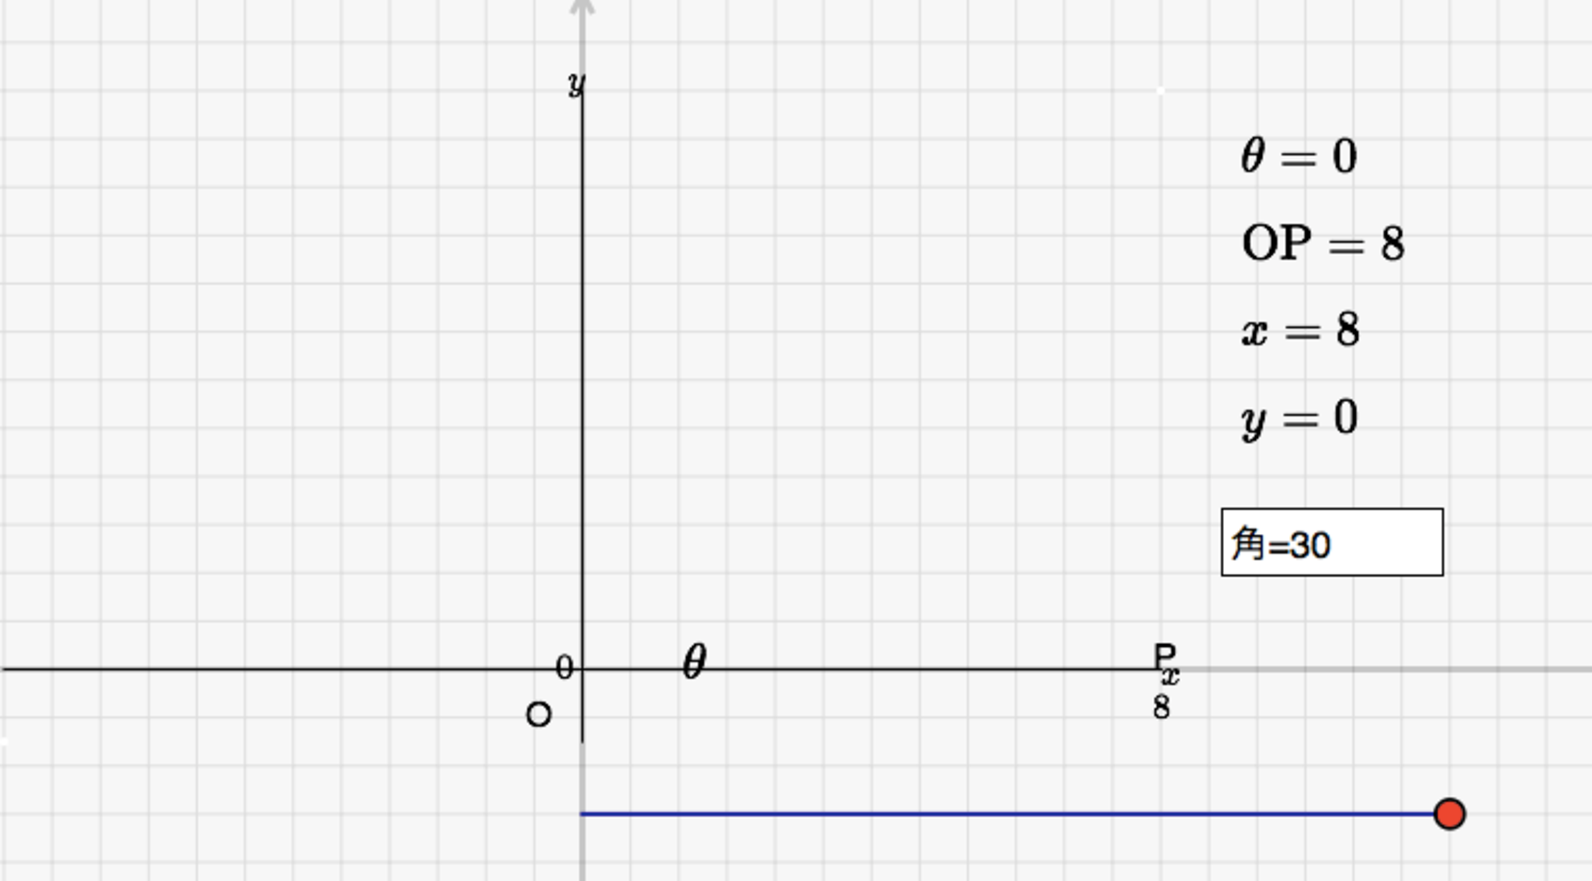
\includegraphics[bb=0.00 0.00 757.00 419.00,width=70mm]{fig/trig0.pdf}}
\end{layer}

\begin{itemize}
\item
[]$\cos\deg{0}=1$
\item
[]$\sin\deg{0}=0$
\item
[]$\tan\deg{0}=0$
\end{itemize}

\newslide{$\deg{90}$の三角比}

\vspace*{18mm}

\slidepage

\begin{layer}{120}{0}
\putnotese{55}{10}{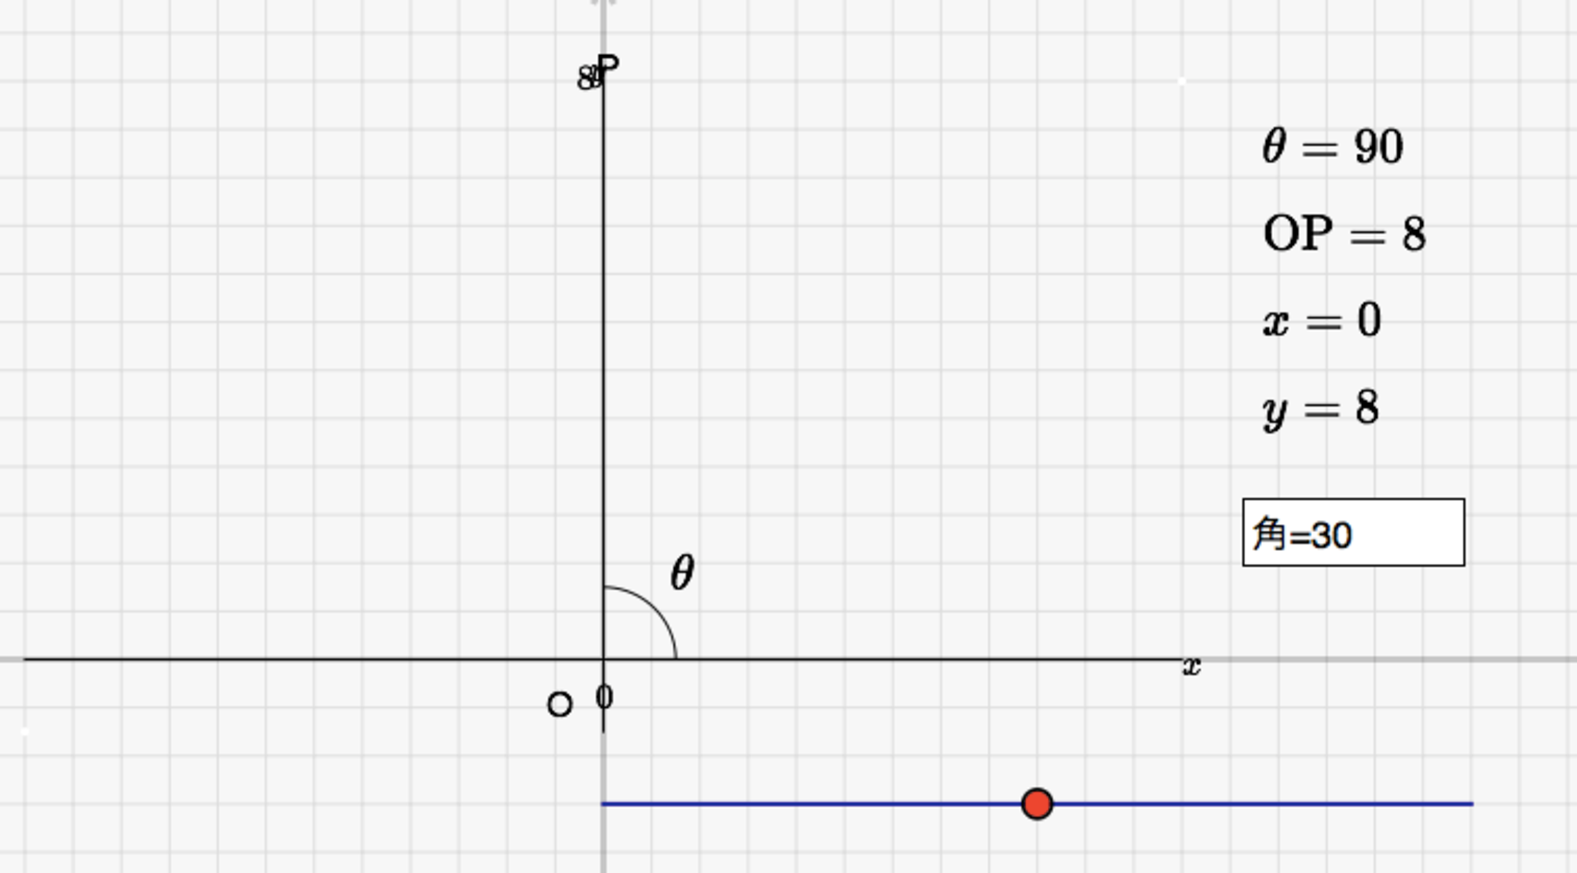
\includegraphics[bb=0.00 0.00 757.00 419.00,width=70mm]{fig/trig90.pdf}}
\end{layer}

\begin{itemize}
\item
[]$\cos\deg{90}=0$
\item
[]$\sin\deg{90}=1$
\item
[]$\tan\deg{90}=\mbox{値がない}$
\end{itemize}

\newslide{鈍角の三角比の符号}

\vspace*{18mm}

\slidepage

\begin{layer}{120}{0}
\putnotese{55}{10}{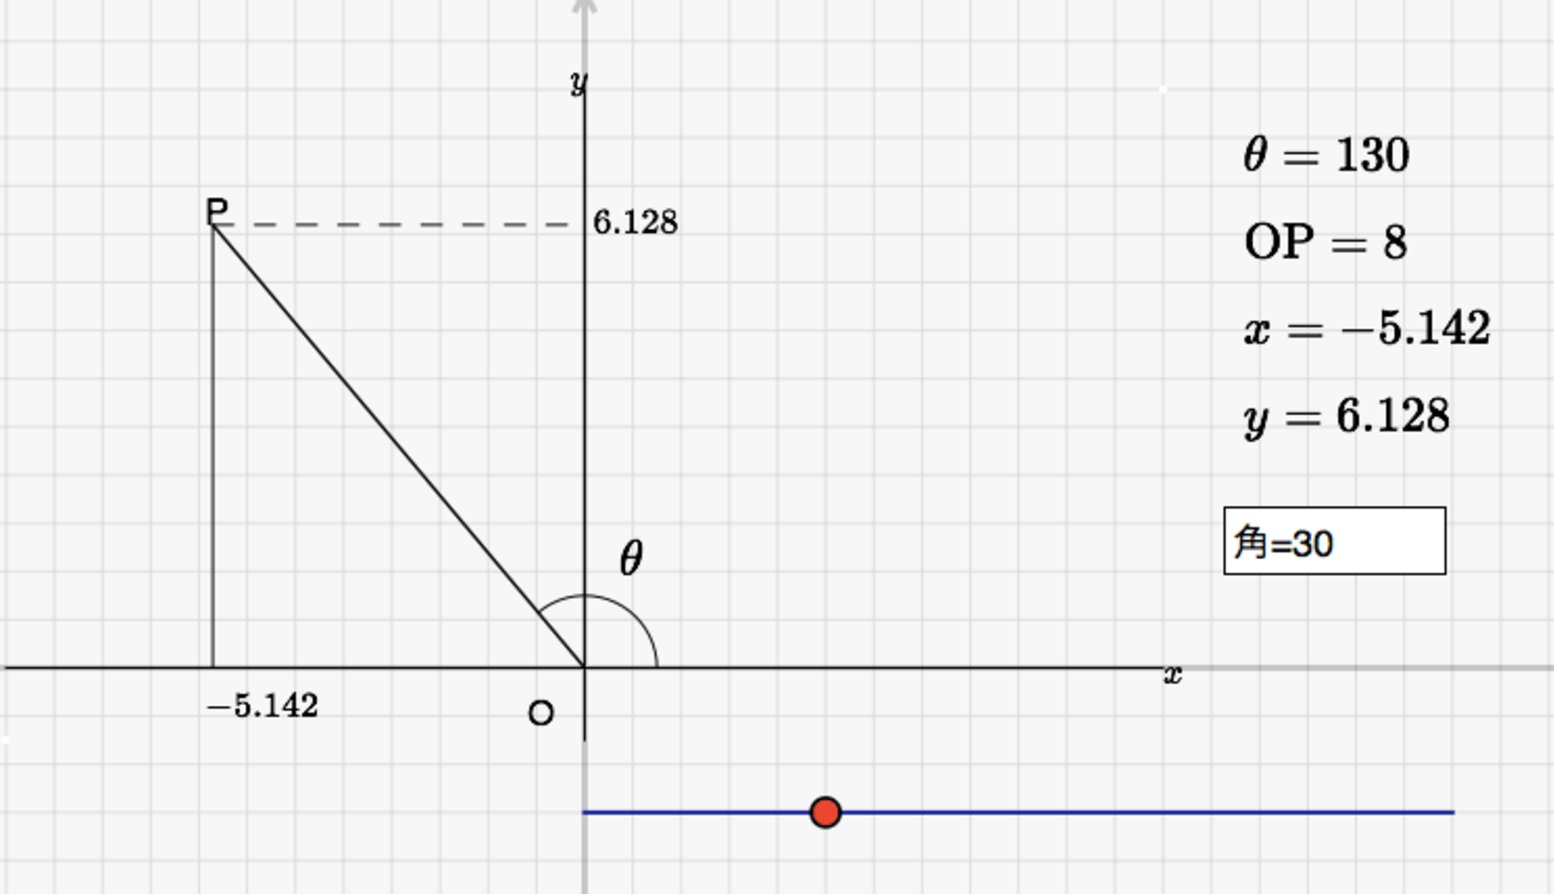
\includegraphics[bb=0.00 0.00 757.00 419.00,width=70mm]{fig/trigobtuse.pdf}}
\end{layer}

\begin{itemize}
\item
[]$\cos$は$-$
\item
[]$\sin$は$+$
\item
[]$\tan$は$-$
\end{itemize}

\newslide{三角比の相互関係}

\vspace*{18mm}

\slidepage

\begin{layer}{120}{0}
\putnotee{60}{40}{\color{red}$\bigl(\cos(\theta)\bigr)^2$を$\cos^2 \theta$と書く}
\putnotese{80}{6}{%%% /Users/takatoosetsuo/Dropbox/2021polytech/103/fig/presen10310305.tex 
%%% Generator=presen103.cdy 
{\unitlength=7mm%
\begin{picture}%
(4.5,3.5)(0,-0.5)%
\special{pn 8}%
%
\Large\bf\boldmath%
\small%
\normalsize%
\special{pn 16}%
\special{pa  1102  -551}\special{pa     0    -0}\special{pa  1102    -0}\special{pa  1102  -551}%
\special{fp}%
\special{pn 8}%
\special{pn 4}%
\special{pa    -0    -0}\special{pa    10     4}\special{pa    19     8}\special{pa    29    12}%
\special{pa    39    16}\special{pa    49    19}\special{pa    59    23}\special{pa    68    26}%
\special{pa    78    30}\special{pa    88    33}\special{pa    98    37}\special{pa   108    40}%
\special{pa   118    43}\special{pa   128    46}\special{pa   138    49}\special{pa   148    52}%
\special{pa   158    55}\special{pa   168    58}\special{pa   179    61}\special{pa   189    64}%
\special{pa   199    66}\special{pa   209    69}\special{pa   219    71}\special{pa   229    74}%
\special{pa   240    76}\special{pa   250    78}\special{pa   260    80}\special{pa   270    82}%
\special{pa   281    84}\special{pa   291    86}\special{pa   301    88}\special{pa   312    90}%
\special{pa   322    92}\special{pa   332    93}\special{pa   343    95}\special{pa   353    96}%
\special{pa   364    98}\special{pa   374    99}\special{pa   384   100}\special{pa   395   102}%
\special{pa   405   103}\special{pa   416   104}\special{pa   426   105}\special{pa   437   106}%
\special{pa   447   106}\special{pa   457   107}\special{pa   468   108}\special{pa   478   108}%
\special{pa   489   109}\special{pa   499   109}\special{pa   510   110}%
\special{fp}%
\special{pa   593   110}\special{pa   603   109}\special{pa   613   109}\special{pa   624   108}%
\special{pa   634   108}\special{pa   645   107}\special{pa   655   106}\special{pa   666   106}%
\special{pa   676   105}\special{pa   687   104}\special{pa   697   103}\special{pa   708   102}%
\special{pa   718   100}\special{pa   728    99}\special{pa   739    98}\special{pa   749    96}%
\special{pa   760    95}\special{pa   770    93}\special{pa   780    92}\special{pa   791    90}%
\special{pa   801    88}\special{pa   811    86}\special{pa   822    84}\special{pa   832    82}%
\special{pa   842    80}\special{pa   852    78}\special{pa   863    76}\special{pa   873    74}%
\special{pa   883    71}\special{pa   893    69}\special{pa   904    66}\special{pa   914    64}%
\special{pa   924    61}\special{pa   934    58}\special{pa   944    55}\special{pa   954    52}%
\special{pa   964    49}\special{pa   974    46}\special{pa   984    43}\special{pa   994    40}%
\special{pa  1004    37}\special{pa  1014    33}\special{pa  1024    30}\special{pa  1034    26}%
\special{pa  1044    23}\special{pa  1054    19}\special{pa  1063    16}\special{pa  1073    12}%
\special{pa  1083     8}\special{pa  1093     4}\special{pa  1102     0}%
\special{fp}%
\special{pn 8}%
\settowidth{\Width}{$x$}\setlength{\Width}{-0.5\Width}%
\settoheight{\Height}{$x$}\settodepth{\Depth}{$x$}\setlength{\Height}{-0.5\Height}\setlength{\Depth}{0.5\Depth}\addtolength{\Height}{\Depth}%
\put(2.0000000,-0.4000000){\hspace*{\Width}\raisebox{\Height}{$x$}}%
%
\special{pn 4}%
\special{pa  1102    -0}\special{pa  1104    -4}\special{pa  1106    -9}\special{pa  1108   -13}%
\special{pa  1110   -18}\special{pa  1111   -22}\special{pa  1113   -27}\special{pa  1115   -32}%
\special{pa  1116   -36}\special{pa  1118   -41}\special{pa  1119   -45}\special{pa  1121   -50}%
\special{pa  1122   -54}\special{pa  1124   -59}\special{pa  1125   -64}\special{pa  1127   -68}%
\special{pa  1128   -73}\special{pa  1130   -77}\special{pa  1131   -82}\special{pa  1132   -87}%
\special{pa  1133   -91}\special{pa  1135   -96}\special{pa  1136  -101}\special{pa  1137  -105}%
\special{pa  1138  -110}\special{pa  1139  -115}\special{pa  1140  -120}\special{pa  1141  -124}%
\special{pa  1142  -129}\special{pa  1143  -134}\special{pa  1144  -138}\special{pa  1145  -143}%
\special{pa  1146  -148}\special{pa  1147  -153}\special{pa  1148  -157}\special{pa  1148  -162}%
\special{pa  1149  -167}\special{pa  1150  -172}\special{pa  1151  -177}\special{pa  1151  -181}%
\special{pa  1152  -186}\special{pa  1152  -191}\special{pa  1153  -196}\special{pa  1154  -201}%
\special{pa  1154  -205}\special{pa  1154  -210}\special{pa  1155  -215}\special{pa  1155  -220}%
\special{pa  1156  -225}\special{pa  1156  -229}\special{pa  1156  -234}%
\special{fp}%
\special{pa  1156  -317}\special{pa  1156  -322}\special{pa  1156  -327}\special{pa  1155  -331}%
\special{pa  1155  -336}\special{pa  1154  -341}\special{pa  1154  -346}\special{pa  1154  -351}%
\special{pa  1153  -355}\special{pa  1152  -360}\special{pa  1152  -365}\special{pa  1151  -370}%
\special{pa  1151  -375}\special{pa  1150  -379}\special{pa  1149  -384}\special{pa  1148  -389}%
\special{pa  1148  -394}\special{pa  1147  -398}\special{pa  1146  -403}\special{pa  1145  -408}%
\special{pa  1144  -413}\special{pa  1143  -417}\special{pa  1142  -422}\special{pa  1141  -427}%
\special{pa  1140  -432}\special{pa  1139  -436}\special{pa  1138  -441}\special{pa  1137  -446}%
\special{pa  1136  -450}\special{pa  1135  -455}\special{pa  1133  -460}\special{pa  1132  -464}%
\special{pa  1131  -469}\special{pa  1130  -474}\special{pa  1128  -478}\special{pa  1127  -483}%
\special{pa  1125  -488}\special{pa  1124  -492}\special{pa  1122  -497}\special{pa  1121  -501}%
\special{pa  1119  -506}\special{pa  1118  -511}\special{pa  1116  -515}\special{pa  1115  -520}%
\special{pa  1113  -524}\special{pa  1111  -529}\special{pa  1110  -533}\special{pa  1108  -538}%
\special{pa  1106  -542}\special{pa  1104  -547}\special{pa  1102  -551}%
\special{fp}%
\special{pn 8}%
\settowidth{\Width}{$y$}\setlength{\Width}{-0.5\Width}%
\settoheight{\Height}{$y$}\settodepth{\Depth}{$y$}\setlength{\Height}{-0.5\Height}\setlength{\Depth}{0.5\Depth}\addtolength{\Height}{\Depth}%
\put(4.2000000,1.0000000){\hspace*{\Width}\raisebox{\Height}{$y$}}%
%
\special{pa  1102   -69}\special{pa  1033   -69}\special{pa  1033    -0}%
\special{fp}%
\special{pa   138    -0}\special{pa   137   -17}\special{pa   133   -34}\special{pa   128   -51}%
\special{pa   123   -62}%
\special{fp}%
\settowidth{\Width}{$\theta$}\setlength{\Width}{-0.5\Width}%
\settoheight{\Height}{$\theta$}\settodepth{\Depth}{$\theta$}\setlength{\Height}{-0.5\Height}\setlength{\Depth}{0.5\Depth}\addtolength{\Height}{\Depth}%
\put(0.9300000,0.2200000){\hspace*{\Width}\raisebox{\Height}{$\theta$}}%
%
\settowidth{\Width}{P}\setlength{\Width}{-0.5\Width}%
\settoheight{\Height}{P}\settodepth{\Depth}{P}\setlength{\Height}{\Depth}%
\put(4.0000000,2.1428571){\hspace*{\Width}\raisebox{\Height}{P}}%
%
\special{pa  1102   -20}\special{pa  1102    20}%
\special{fp}%
\settowidth{\Width}{$x$}\setlength{\Width}{-0.5\Width}%
\settoheight{\Height}{$x$}\settodepth{\Depth}{$x$}\setlength{\Height}{-\Height}%
\put(4.0000000,-0.1428571){\hspace*{\Width}\raisebox{\Height}{$x$}}%
%
\special{pa    20  -551}\special{pa     0  -551}%
\special{fp}%
\settowidth{\Width}{$y$}\setlength{\Width}{-1\Width}%
\settoheight{\Height}{$y$}\settodepth{\Depth}{$y$}\setlength{\Height}{-0.5\Height}\setlength{\Depth}{0.5\Depth}\addtolength{\Height}{\Depth}%
\put(-0.1428571,2.0000000){\hspace*{\Width}\raisebox{\Height}{$y$}}%
%
\special{pa     0    -0}\special{pa  1240    -0}%
\special{fp}%
\special{pa     0   138}\special{pa     0  -827}%
\special{fp}%
\settowidth{\Width}{$x$}\setlength{\Width}{0\Width}%
\settoheight{\Height}{$x$}\settodepth{\Depth}{$x$}\setlength{\Height}{-0.5\Height}\setlength{\Depth}{0.5\Depth}\addtolength{\Height}{\Depth}%
\put(4.5714286,0.0000000){\hspace*{\Width}\raisebox{\Height}{$x$}}%
%
\settowidth{\Width}{$y$}\setlength{\Width}{-0.5\Width}%
\settoheight{\Height}{$y$}\settodepth{\Depth}{$y$}\setlength{\Height}{\Depth}%
\put(0.0000000,3.0714286){\hspace*{\Width}\raisebox{\Height}{$y$}}%
%
\settowidth{\Width}{O}\setlength{\Width}{-1\Width}%
\settoheight{\Height}{O}\settodepth{\Depth}{O}\setlength{\Height}{-\Height}%
\put(-0.0714286,-0.0714286){\hspace*{\Width}\raisebox{\Height}{O}}%
%
\end{picture}}%}
\end{layer}

\begin{itemize}
\item
[(1)\ ]$\tan\theta=\bunsuu{\sin\theta}{\cos\theta}$
\item
[\color{blue}証)]{\color{blue}$\tan\theta=\bunsuu{y}{x}=\bunsuu{\frac{y}{\mathrm{OP}}}{\frac{x}{\mathrm{OP}}}$}
{\color{blue}$=\bunsuu{\sin\theta}{\cos\theta}$}
\item
[(2)\ ]$\cos^2\theta+\sin^2\theta=1$
\item
[\color{blue}証)]{\color{blue}$\cos^2\theta+\sin^2\theta=\bunsuu{x^2}{\mathrm{OP}^2}+\bunsuu{y^2}{\mathrm{OP}^2}$}
{\color{blue}$=\bunsuu{x^2+y^2}{\mathrm{OP^2}}=1$}
\end{itemize}

\newslide{課題(三角比の相互関係)}

\vspace*{18mm}

%%repeat=1
\slidepage
\vspace{4mm}

\begin{itemize}
\item
[課題]\monban $\cos\theta=\bunsuu{1}{3}$のとき,$\sin\theta$を求めよ.ただし,$\theta$は鋭角とする\hfill TextP107
\item
[課題]\monban $\sin\theta=\bunsuu{2}{3}$とする.次の場合のそれぞれについて$\cos\theta$を求めよ\vspace{2mm}\seteda{55}\\
\eda{$\theta$が鋭角のとき}\eda{$\theta$が鈍角のとき}
\end{itemize}
%%%%%%%%%%%%

%%%%%%%%%%%%%%%%%%%%

\mainslide{一般角}


\slidepage[m]
%%%%%%%%%%%%

%%%%%%%%%%%%%%%%%%%%

\newslide{一般角}

\vspace*{18mm}

\slidepage

\begin{layer}{120}{0}
\putnotese{78}{17}{%%% /Users/takatoosetsuo/Dropbox/2019polytec/lectures/0527/presen/fig/generalanglen30.tex 
%%% Generator=generalangle.cdy 
{\unitlength=1cm%
\begin{picture}%
(5,5)(-2.5,-2.5)%
\special{pn 8}%
%
\normalsize%
\special{pn 12}%
\special{pa   787    -0}\special{pa   781   -99}\special{pa   763  -196}\special{pa   732  -290}%
\special{pa   690  -379}\special{pa   637  -463}\special{pa   574  -539}\special{pa   502  -607}%
\special{pa   422  -665}\special{pa   335  -712}\special{pa   243  -749}\special{pa   148  -773}%
\special{pa    49  -786}\special{pa   -49  -786}\special{pa  -148  -773}\special{pa  -243  -749}%
\special{pa  -335  -712}\special{pa  -422  -665}\special{pa  -502  -607}\special{pa  -574  -539}%
\special{pa  -637  -463}\special{pa  -690  -379}\special{pa  -732  -290}\special{pa  -763  -196}%
\special{pa  -781   -99}\special{pa  -787     0}\special{pa  -781    99}\special{pa  -763   196}%
\special{pa  -732   290}\special{pa  -690   379}\special{pa  -637   463}\special{pa  -574   539}%
\special{pa  -502   607}\special{pa  -422   665}\special{pa  -335   712}\special{pa  -243   749}%
\special{pa  -148   773}\special{pa   -49   786}\special{pa    49   786}\special{pa   148   773}%
\special{pa   243   749}\special{pa   335   712}\special{pa   422   665}\special{pa   502   607}%
\special{pa   574   539}\special{pa   637   463}\special{pa   690   379}\special{pa   732   290}%
\special{pa   763   196}\special{pa   781    99}\special{pa   787     0}%
\special{fp}%
\special{pn 8}%
\special{pn 12}%
\special{pa   787    -0}\special{pa   781   -99}\special{pa   763  -196}\special{pa   732  -290}%
\special{pa   690  -379}\special{pa   637  -463}\special{pa   574  -539}\special{pa   502  -607}%
\special{pa   422  -665}\special{pa   335  -712}\special{pa   243  -749}\special{pa   148  -773}%
\special{pa    49  -786}\special{pa   -49  -786}\special{pa  -148  -773}\special{pa  -243  -749}%
\special{pa  -335  -712}\special{pa  -422  -665}\special{pa  -502  -607}\special{pa  -574  -539}%
\special{pa  -637  -463}\special{pa  -690  -379}\special{pa  -732  -290}\special{pa  -763  -196}%
\special{pa  -781   -99}\special{pa  -787     0}\special{pa  -781    99}\special{pa  -763   196}%
\special{pa  -732   290}\special{pa  -690   379}\special{pa  -637   463}\special{pa  -574   539}%
\special{pa  -502   607}\special{pa  -422   665}\special{pa  -335   712}\special{pa  -243   749}%
\special{pa  -148   773}\special{pa   -49   786}\special{pa    49   786}\special{pa   148   773}%
\special{pa   243   749}\special{pa   335   712}\special{pa   422   665}\special{pa   502   607}%
\special{pa   574   539}\special{pa   637   463}\special{pa   690   379}\special{pa   732   290}%
\special{pa   763   196}\special{pa   781    99}\special{pa   787     0}%
\special{fp}%
\special{pn 8}%
{\special{pn 0}\color[rgb]{0,0,0}%
\special{pa 699 377}\special{pa 691 372}\special{pa 683 370}\special{pa 674 371}\special{pa 667 376}\special{pa 661 382}\special{pa 659 390}\special{pa 659 399}\special{pa 662 407}\special{pa 669 413}\special{pa 677 417}\special{pa 685 417}\special{pa 693 414}\special{pa 700 409}\special{pa 704 401}\special{pa 706 393}\special{pa 704 384}\special{pa 699 377}\special{sh}\special{fp}}%
\special{pn 4}\special{pa 699 377}\special{pa 691 372}\special{pa 683 370}\special{pa 674 371}\special{pa 667 376}\special{pa 661 382}\special{pa 659 390}\special{pa 659 399}\special{pa 662 407}\special{pa 669 413}\special{pa 677 417}\special{pa 685 417}\special{pa 693 414}\special{pa 700 409}\special{pa 704 401}\special{pa 706 393}\special{pa 704 384}\special{pa 699 377}\special{fp}%
\settowidth{\Width}{$(\sqrt{3},-1)$}\setlength{\Width}{0\Width}%
\settoheight{\Height}{$(\sqrt{3},-1)$}\settodepth{\Depth}{$(\sqrt{3},-1)$}\setlength{\Height}{-\Height}%
\put(1.7800000,-1.0500000){\hspace*{\Width}\raisebox{\Height}{$(\sqrt{3},-1)$}}%
%
\special{pa   787   -20}\special{pa   787    20}%
\special{fp}%
\settowidth{\Width}{$2$}\setlength{\Width}{0\Width}%
\settoheight{\Height}{$2$}\settodepth{\Depth}{$2$}\setlength{\Height}{-\Height}%
\put(2.0500000,-0.0500000){\hspace*{\Width}\raisebox{\Height}{$2$}}%
%
{%
\color[rgb]{1,0,0}%
\special{pn 12}%
\special{pa     0    -0}\special{pa   682   394}%
\special{fp}%
\special{pn 8}%
}%
\special{pa   197    -0}\special{pa   197     2}\special{pa   197     4}\special{pa   197     6}%
\special{pa   197     8}\special{pa   197    10}\special{pa   197    12}\special{pa   197    14}%
\special{pa   197    17}\special{pa   197    19}\special{pa   196    21}\special{pa   196    23}%
\special{pa   196    25}\special{pa   196    27}\special{pa   196    29}\special{pa   195    31}%
\special{pa   195    33}\special{pa   195    35}\special{pa   195    37}\special{pa   194    39}%
\special{pa   194    41}\special{pa   193    43}\special{pa   193    45}\special{pa   193    47}%
\special{pa   192    49}\special{pa   192    51}\special{pa   191    53}\special{pa   191    55}%
\special{pa   190    57}\special{pa   190    59}\special{pa   189    61}\special{pa   188    63}%
\special{pa   188    65}\special{pa   187    67}\special{pa   187    69}\special{pa   186    71}%
\special{pa   185    73}\special{pa   185    75}\special{pa   184    77}\special{pa   183    79}%
\special{pa   182    81}\special{pa   181    83}\special{pa   181    85}\special{pa   180    87}%
\special{pa   179    89}\special{pa   178    91}\special{pa   177    93}\special{pa   176    94}%
\special{pa   175    96}\special{pa   174    98}\special{pa   173   100}%
\special{fp}%
\special{pa 177 61}\special{pa 173 100}\special{pa 199 70}\special{pa 188 66}\special{pa 177 61}%
\special{pa 177 61}\special{sh 1}\special{ip}%
\special{pn 1}%
\special{pa   177    61}\special{pa   173   100}\special{pa   199    70}\special{pa   188    66}%
\special{pa   177    61}\special{pa   173   100}%
\special{fp}%
\special{pn 8}%
\settowidth{\Width}{$\theta=-30^{\circ}$}\setlength{\Width}{0\Width}%
\settoheight{\Height}{$\theta=-30^{\circ}$}\settodepth{\Depth}{$\theta=-30^{\circ}$}\setlength{\Height}{-0.5\Height}\setlength{\Depth}{0.5\Depth}\addtolength{\Height}{\Depth}%
\put(-1.4500000,1.0000000){\hspace*{\Width}\raisebox{\Height}{$\theta=-30^{\circ}$}}%
%
\special{pa  -984    -0}\special{pa   984    -0}%
\special{fp}%
\special{pa     0   984}\special{pa     0  -984}%
\special{fp}%
\settowidth{\Width}{$x$}\setlength{\Width}{0\Width}%
\settoheight{\Height}{$x$}\settodepth{\Depth}{$x$}\setlength{\Height}{-0.5\Height}\setlength{\Depth}{0.5\Depth}\addtolength{\Height}{\Depth}%
\put(2.5500000,0.0000000){\hspace*{\Width}\raisebox{\Height}{$x$}}%
%
\settowidth{\Width}{$y$}\setlength{\Width}{-0.5\Width}%
\settoheight{\Height}{$y$}\settodepth{\Depth}{$y$}\setlength{\Height}{\Depth}%
\put(0.0000000,2.5500000){\hspace*{\Width}\raisebox{\Height}{$y$}}%
%
\settowidth{\Width}{O}\setlength{\Width}{-1\Width}%
\settoheight{\Height}{O}\settodepth{\Depth}{O}\setlength{\Height}{-\Height}%
\put(-0.0500000,-0.0500000){\hspace*{\Width}\raisebox{\Height}{O}}%
%
\end{picture}}%}
\end{layer}

\begin{itemize}
\item
これまで,角$\theta$は2つの線分の間の角だった\\
\hspace*{2zw}$0^{\circ} \leqq \theta \leqq 360^{\circ}$
\item
角を回転を表す量とすると\\
$\theta$はどんな実数でもよい.
\begin{itemize}
\item
[$\cdot$]$x$軸を始線とする
\item
[$\cdot$]$\theta >0^{\circ}$のとき,反時計回り
\item
[$\cdot$]$\theta<0^{\circ}$のとき,時計回り
\end{itemize}
\end{itemize}

\newslide{一般角}

\vspace*{18mm}

\slidepage

\begin{layer}{120}{0}
\putnotese{85}{20}{\scalebox{0.7}{%%% /Users/takatoosetsuo/Dropbox/2021polytech/103/fig/presen103xy.tex 
%%% Generator=presen103.cdy 
{\unitlength=6mm%
\begin{picture}%
(10,10)(-5,-5)%
\special{pn 8}%
%
\Large\bf\boldmath%
\small%
\special{pa -1181    -0}\special{pa  1181    -0}%
\special{fp}%
\special{pa     0  1181}\special{pa     0 -1181}%
\special{fp}%
\settowidth{\Width}{$x$}\setlength{\Width}{0\Width}%
\settoheight{\Height}{$x$}\settodepth{\Depth}{$x$}\setlength{\Height}{-0.5\Height}\setlength{\Depth}{0.5\Depth}\addtolength{\Height}{\Depth}%
\put(5.0833333,0.0000000){\hspace*{\Width}\raisebox{\Height}{$x$}}%
%
\settowidth{\Width}{$y$}\setlength{\Width}{-0.5\Width}%
\settoheight{\Height}{$y$}\settodepth{\Depth}{$y$}\setlength{\Height}{\Depth}%
\put(0.0000000,5.0833333){\hspace*{\Width}\raisebox{\Height}{$y$}}%
%
\settowidth{\Width}{O}\setlength{\Width}{-1\Width}%
\settoheight{\Height}{O}\settodepth{\Depth}{O}\setlength{\Height}{-\Height}%
\put(-0.0833333,-0.0833333){\hspace*{\Width}\raisebox{\Height}{O}}%
%
\end{picture}}%}}
\putnotec{115}{30}{\normalsize\color{red}第1象限}
\putnotec{95}{30}{\normalsize\color{red}第2象限}
\putnotec{95}{52}{\normalsize\color{red}第3象限}
\putnotec{115}{52}{\normalsize\color{red}第4象限}
\end{layer}

\vspace*{5mm}

\noindent
HTML「一般角」で一般角を見てみよう
\begin{itemize}
\item
[課題]\monban 次の角は第何象限にあるか.\seteda{40}\\
\eda{$\deg{400}$}\eda{$\deg{600}$}\\
\eda{$\deg{-500}$}\eda{$\deg{-700}$}
\end{itemize}

\newslide{一般角の三角比}

\vspace*{18mm}

\slidepage

\begin{layer}{120}{0}
\putnotese{75}{17}{%%% /Users/takatoosetsuo/Dropbox/2019polytec/lectures/0527/presen/fig/generalanglen30.tex 
%%% Generator=generalangle.cdy 
{\unitlength=1cm%
\begin{picture}%
(5,5)(-2.5,-2.5)%
\special{pn 8}%
%
\normalsize%
\special{pn 12}%
\special{pa   787    -0}\special{pa   781   -99}\special{pa   763  -196}\special{pa   732  -290}%
\special{pa   690  -379}\special{pa   637  -463}\special{pa   574  -539}\special{pa   502  -607}%
\special{pa   422  -665}\special{pa   335  -712}\special{pa   243  -749}\special{pa   148  -773}%
\special{pa    49  -786}\special{pa   -49  -786}\special{pa  -148  -773}\special{pa  -243  -749}%
\special{pa  -335  -712}\special{pa  -422  -665}\special{pa  -502  -607}\special{pa  -574  -539}%
\special{pa  -637  -463}\special{pa  -690  -379}\special{pa  -732  -290}\special{pa  -763  -196}%
\special{pa  -781   -99}\special{pa  -787     0}\special{pa  -781    99}\special{pa  -763   196}%
\special{pa  -732   290}\special{pa  -690   379}\special{pa  -637   463}\special{pa  -574   539}%
\special{pa  -502   607}\special{pa  -422   665}\special{pa  -335   712}\special{pa  -243   749}%
\special{pa  -148   773}\special{pa   -49   786}\special{pa    49   786}\special{pa   148   773}%
\special{pa   243   749}\special{pa   335   712}\special{pa   422   665}\special{pa   502   607}%
\special{pa   574   539}\special{pa   637   463}\special{pa   690   379}\special{pa   732   290}%
\special{pa   763   196}\special{pa   781    99}\special{pa   787     0}%
\special{fp}%
\special{pn 8}%
\special{pn 12}%
\special{pa   787    -0}\special{pa   781   -99}\special{pa   763  -196}\special{pa   732  -290}%
\special{pa   690  -379}\special{pa   637  -463}\special{pa   574  -539}\special{pa   502  -607}%
\special{pa   422  -665}\special{pa   335  -712}\special{pa   243  -749}\special{pa   148  -773}%
\special{pa    49  -786}\special{pa   -49  -786}\special{pa  -148  -773}\special{pa  -243  -749}%
\special{pa  -335  -712}\special{pa  -422  -665}\special{pa  -502  -607}\special{pa  -574  -539}%
\special{pa  -637  -463}\special{pa  -690  -379}\special{pa  -732  -290}\special{pa  -763  -196}%
\special{pa  -781   -99}\special{pa  -787     0}\special{pa  -781    99}\special{pa  -763   196}%
\special{pa  -732   290}\special{pa  -690   379}\special{pa  -637   463}\special{pa  -574   539}%
\special{pa  -502   607}\special{pa  -422   665}\special{pa  -335   712}\special{pa  -243   749}%
\special{pa  -148   773}\special{pa   -49   786}\special{pa    49   786}\special{pa   148   773}%
\special{pa   243   749}\special{pa   335   712}\special{pa   422   665}\special{pa   502   607}%
\special{pa   574   539}\special{pa   637   463}\special{pa   690   379}\special{pa   732   290}%
\special{pa   763   196}\special{pa   781    99}\special{pa   787     0}%
\special{fp}%
\special{pn 8}%
{\special{pn 0}\color[rgb]{0,0,0}%
\special{pa 699 377}\special{pa 691 372}\special{pa 683 370}\special{pa 674 371}\special{pa 667 376}\special{pa 661 382}\special{pa 659 390}\special{pa 659 399}\special{pa 662 407}\special{pa 669 413}\special{pa 677 417}\special{pa 685 417}\special{pa 693 414}\special{pa 700 409}\special{pa 704 401}\special{pa 706 393}\special{pa 704 384}\special{pa 699 377}\special{sh}\special{fp}}%
\special{pn 4}\special{pa 699 377}\special{pa 691 372}\special{pa 683 370}\special{pa 674 371}\special{pa 667 376}\special{pa 661 382}\special{pa 659 390}\special{pa 659 399}\special{pa 662 407}\special{pa 669 413}\special{pa 677 417}\special{pa 685 417}\special{pa 693 414}\special{pa 700 409}\special{pa 704 401}\special{pa 706 393}\special{pa 704 384}\special{pa 699 377}\special{fp}%
\settowidth{\Width}{$(\sqrt{3},-1)$}\setlength{\Width}{0\Width}%
\settoheight{\Height}{$(\sqrt{3},-1)$}\settodepth{\Depth}{$(\sqrt{3},-1)$}\setlength{\Height}{-\Height}%
\put(1.7800000,-1.0500000){\hspace*{\Width}\raisebox{\Height}{$(\sqrt{3},-1)$}}%
%
\special{pa   787   -20}\special{pa   787    20}%
\special{fp}%
\settowidth{\Width}{$2$}\setlength{\Width}{0\Width}%
\settoheight{\Height}{$2$}\settodepth{\Depth}{$2$}\setlength{\Height}{-\Height}%
\put(2.0500000,-0.0500000){\hspace*{\Width}\raisebox{\Height}{$2$}}%
%
{%
\color[rgb]{1,0,0}%
\special{pn 12}%
\special{pa     0    -0}\special{pa   682   394}%
\special{fp}%
\special{pn 8}%
}%
\special{pa   197    -0}\special{pa   197     2}\special{pa   197     4}\special{pa   197     6}%
\special{pa   197     8}\special{pa   197    10}\special{pa   197    12}\special{pa   197    14}%
\special{pa   197    17}\special{pa   197    19}\special{pa   196    21}\special{pa   196    23}%
\special{pa   196    25}\special{pa   196    27}\special{pa   196    29}\special{pa   195    31}%
\special{pa   195    33}\special{pa   195    35}\special{pa   195    37}\special{pa   194    39}%
\special{pa   194    41}\special{pa   193    43}\special{pa   193    45}\special{pa   193    47}%
\special{pa   192    49}\special{pa   192    51}\special{pa   191    53}\special{pa   191    55}%
\special{pa   190    57}\special{pa   190    59}\special{pa   189    61}\special{pa   188    63}%
\special{pa   188    65}\special{pa   187    67}\special{pa   187    69}\special{pa   186    71}%
\special{pa   185    73}\special{pa   185    75}\special{pa   184    77}\special{pa   183    79}%
\special{pa   182    81}\special{pa   181    83}\special{pa   181    85}\special{pa   180    87}%
\special{pa   179    89}\special{pa   178    91}\special{pa   177    93}\special{pa   176    94}%
\special{pa   175    96}\special{pa   174    98}\special{pa   173   100}%
\special{fp}%
\special{pa 177 61}\special{pa 173 100}\special{pa 199 70}\special{pa 188 66}\special{pa 177 61}%
\special{pa 177 61}\special{sh 1}\special{ip}%
\special{pn 1}%
\special{pa   177    61}\special{pa   173   100}\special{pa   199    70}\special{pa   188    66}%
\special{pa   177    61}\special{pa   173   100}%
\special{fp}%
\special{pn 8}%
\settowidth{\Width}{$\theta=-30^{\circ}$}\setlength{\Width}{0\Width}%
\settoheight{\Height}{$\theta=-30^{\circ}$}\settodepth{\Depth}{$\theta=-30^{\circ}$}\setlength{\Height}{-0.5\Height}\setlength{\Depth}{0.5\Depth}\addtolength{\Height}{\Depth}%
\put(-1.4500000,1.0000000){\hspace*{\Width}\raisebox{\Height}{$\theta=-30^{\circ}$}}%
%
\special{pa  -984    -0}\special{pa   984    -0}%
\special{fp}%
\special{pa     0   984}\special{pa     0  -984}%
\special{fp}%
\settowidth{\Width}{$x$}\setlength{\Width}{0\Width}%
\settoheight{\Height}{$x$}\settodepth{\Depth}{$x$}\setlength{\Height}{-0.5\Height}\setlength{\Depth}{0.5\Depth}\addtolength{\Height}{\Depth}%
\put(2.5500000,0.0000000){\hspace*{\Width}\raisebox{\Height}{$x$}}%
%
\settowidth{\Width}{$y$}\setlength{\Width}{-0.5\Width}%
\settoheight{\Height}{$y$}\settodepth{\Depth}{$y$}\setlength{\Height}{\Depth}%
\put(0.0000000,2.5500000){\hspace*{\Width}\raisebox{\Height}{$y$}}%
%
\settowidth{\Width}{O}\setlength{\Width}{-1\Width}%
\settoheight{\Height}{O}\settodepth{\Depth}{O}\setlength{\Height}{-\Height}%
\put(-0.0500000,-0.0500000){\hspace*{\Width}\raisebox{\Height}{O}}%
%
\end{picture}}%}
\end{layer}

\begin{itemize}
\item
座標を使う(鈍角の場合と同じ)\vspace{-1mm}
\item
[例]$\theta=-30^{\circ}$\\
\hspace*{1zw}$\cos\theta=$\\
\hspace*{1zw}$\sin\theta=$\\
\hspace*{1zw}$\tan\theta=$\vspace{-1mm}
\item
[課題]\monban 次の値を求めよ.\seteda{35}\\
\eda{$\cos 240\degree$}\eda{$\sin 240\degree$}\\
\eda{$\sin(-30\degree)$}\eda{$\tan(-30\degree)$}
\end{itemize}
\ifnum 1=0

\mainslide{弧度法(radian)}


\slidepage[m]
%%%%%%%%%%%%

%%%%%%%%%%%%%%%%%%%%

\newslide{角度の測り方1}

\vspace*{18mm}

\slidepage

\begin{layer}{120}{0}
\putnotese{90}{10}{%%% /polytech.git/n102/fig/kakudo001.tex 
%%% Generator=presen0609.cdy 
{\unitlength=1cm%
\begin{picture}%
(4,4)(-2,-2)%
\special{pn 8}%
%
\Large\bf\boldmath%
\small%
{%
\color[rgb]{0,0,0}%
\special{pa   787    -0}\special{pa   781   -99}\special{pa   763  -196}\special{pa   732  -290}%
\special{pa   690  -379}\special{pa   637  -463}\special{pa   574  -539}\special{pa   502  -607}%
\special{pa   422  -665}\special{pa   335  -712}\special{pa   243  -749}\special{pa   148  -773}%
\special{pa    49  -786}\special{pa   -49  -786}\special{pa  -148  -773}\special{pa  -243  -749}%
\special{pa  -335  -712}\special{pa  -422  -665}\special{pa  -502  -607}\special{pa  -574  -539}%
\special{pa  -637  -463}\special{pa  -690  -379}\special{pa  -732  -290}\special{pa  -763  -196}%
\special{pa  -781   -99}\special{pa  -787     0}\special{pa  -781    99}\special{pa  -763   196}%
\special{pa  -732   290}\special{pa  -690   379}\special{pa  -637   463}\special{pa  -574   539}%
\special{pa  -502   607}\special{pa  -422   665}\special{pa  -335   712}\special{pa  -243   749}%
\special{pa  -148   773}\special{pa   -49   786}\special{pa    49   786}\special{pa   148   773}%
\special{pa   243   749}\special{pa   335   712}\special{pa   422   665}\special{pa   502   607}%
\special{pa   574   539}\special{pa   637   463}\special{pa   690   379}\special{pa   732   290}%
\special{pa   763   196}\special{pa   781    99}\special{pa   787     0}%
\special{fp}%
}%
{%
\color[rgb]{0,0,0}%
\special{pa     0    -0}\special{pa   787    -0}%
\special{fp}%
}%
{%
\color[rgb]{0,0,0}%
\special{pa     0    -0}\special{pa   787   -14}%
\special{fp}%
}%
{%
\color[rgb]{0,0,0}%
\settowidth{\Width}{$\theta=1^{\circ}$}\setlength{\Width}{-0.5\Width}%
\settoheight{\Height}{$\theta=1^{\circ}$}\settodepth{\Depth}{$\theta=1^{\circ}$}\setlength{\Height}{\Depth}%
\put(1.0000000,0.2200000){\hspace*{\Width}\raisebox{\Height}{$\theta=1^{\circ}$}}%
%
}%
\end{picture}}%}
\end{layer}

\noindent
度 ${}^{\circ}$\vspace{-1mm}
\begin{itemize}
\item
1周を$360^{\circ}$とする
\item
半周は$180^{\circ}$とする
\item
一周の$\bunsuu{1}{360}$を$1^{\circ}$とする
\item
数学的な意味は余りない
\item
日常的には使いやすい
\end{itemize}

\newslide{角度の測り方2(弧度法)}

\vspace*{18mm}


\begin{layer}{120}{0}
\putnotew{96}{73}{\hyperlink{para0pg5}{\fbox{\Ctab{2.5mm}{\scalebox{1}{\scriptsize $\mathstrut||\!\lhd$}}}}}
\putnotew{101}{73}{\hyperlink{para1pg1}{\fbox{\Ctab{2.5mm}{\scalebox{1}{\scriptsize $\mathstrut|\!\lhd$}}}}}
\putnotew{108}{73}{\hyperlink{para1pg4}{\fbox{\Ctab{4.5mm}{\scalebox{1}{\scriptsize $\mathstrut\!\!\lhd\!\!$}}}}}
\putnotew{115}{73}{\hyperlink{para1pg5}{\fbox{\Ctab{4.5mm}{\scalebox{1}{\scriptsize $\mathstrut\!\rhd\!$}}}}}
\putnotew{120}{73}{\hyperlink{para1pg5}{\fbox{\Ctab{2.5mm}{\scalebox{1}{\scriptsize $\mathstrut \!\rhd\!\!|$}}}}}
\putnotew{125}{73}{\hyperlink{para2pg1}{\fbox{\Ctab{2.5mm}{\scalebox{1}{\scriptsize $\mathstrut \!\rhd\!\!||$}}}}}
\putnotee{126}{73}{\scriptsize\color{blue} 5/5}
\end{layer}

\slidepage

\begin{layer}{120}{0}
\putnotese{87}{10}{%%% /Users/takatoosetsuo/Dropbox/2018polytec/lecture/0514/presen/fig/radian.tex 
%%% Generator=presen0514.cdy 
{\unitlength=1cm%
\begin{picture}%
(4.35,4.12)(-2.06,-2.06)%
\special{pn 8}%
%
\Large\bf\boldmath%
\small%
\special{pn 12}%
\special{pa   787    -0}\special{pa     0    -0}\special{pa   475  -628}%
\special{fp}%
\special{pn 8}%
\special{pn 8}%
\special{pa 788 4}\special{pa 787 -4}\special{fp}\special{pa 786 -35}\special{pa 786 -43}\special{fp}%
\special{pa 784 -74}\special{pa 783 -82}\special{fp}\special{pa 779 -113}\special{pa 778 -121}\special{fp}%
\special{pa 772 -152}\special{pa 771 -160}\special{fp}\special{pa 764 -190}\special{pa 762 -198}\special{fp}%
\special{pa 753 -228}\special{pa 751 -236}\special{fp}\special{pa 741 -265}\special{pa 738 -273}\special{fp}%
\special{pa 727 -302}\special{pa 724 -309}\special{fp}\special{pa 711 -338}\special{pa 708 -345}\special{fp}%
\special{pa 693 -373}\special{pa 690 -380}\special{fp}\special{pa 674 -407}\special{pa 670 -414}\special{fp}%
\special{pa 653 -440}\special{pa 648 -447}\special{fp}\special{pa 630 -472}\special{pa 625 -478}\special{fp}%
\special{pa 606 -503}\special{pa 601 -509}\special{fp}\special{pa 580 -533}\special{pa 574 -538}\special{fp}%
\special{pa 552 -561}\special{pa 547 -566}\special{fp}\special{pa 524 -587}\special{pa 518 -593}\special{fp}%
\special{pa 494 -613}\special{pa 488 -618}\special{fp}\special{pa 463 -637}\special{pa 456 -642}\special{fp}%
\special{pa 430 -659}\special{pa 424 -663}\special{fp}\special{pa 397 -680}\special{pa 390 -684}\special{fp}%
\special{pa 363 -699}\special{pa 355 -702}\special{fp}\special{pa 327 -716}\special{pa 320 -719}\special{fp}%
\special{pa 291 -731}\special{pa 284 -734}\special{fp}\special{pa 255 -745}\special{pa 247 -747}\special{fp}%
\special{pa 217 -757}\special{pa 209 -759}\special{fp}\special{pa 179 -766}\special{pa 171 -768}\special{fp}%
\special{pa 141 -774}\special{pa 133 -776}\special{fp}\special{pa 102 -781}\special{pa 94 -782}\special{fp}%
\special{pa 63 -785}\special{pa 55 -785}\special{fp}\special{pa 24 -787}\special{pa 16 -787}\special{fp}%
\special{pa -16 -787}\special{pa -24 -787}\special{fp}\special{pa -55 -785}\special{pa -63 -785}\special{fp}%
\special{pa -94 -782}\special{pa -102 -781}\special{fp}\special{pa -133 -776}\special{pa -141 -774}\special{fp}%
\special{pa -171 -768}\special{pa -179 -766}\special{fp}\special{pa -209 -759}\special{pa -217 -757}\special{fp}%
\special{pa -247 -747}\special{pa -255 -745}\special{fp}\special{pa -284 -734}\special{pa -291 -731}\special{fp}%
\special{pa -320 -719}\special{pa -327 -716}\special{fp}\special{pa -355 -702}\special{pa -363 -699}\special{fp}%
\special{pa -390 -684}\special{pa -397 -680}\special{fp}\special{pa -424 -663}\special{pa -430 -659}\special{fp}%
\special{pa -456 -642}\special{pa -463 -637}\special{fp}\special{pa -488 -618}\special{pa -494 -613}\special{fp}%
\special{pa -518 -593}\special{pa -524 -587}\special{fp}\special{pa -547 -566}\special{pa -552 -561}\special{fp}%
\special{pa -574 -538}\special{pa -580 -533}\special{fp}\special{pa -601 -509}\special{pa -606 -503}\special{fp}%
\special{pa -625 -478}\special{pa -630 -472}\special{fp}\special{pa -648 -447}\special{pa -653 -440}\special{fp}%
\special{pa -670 -414}\special{pa -674 -407}\special{fp}\special{pa -690 -380}\special{pa -693 -373}\special{fp}%
\special{pa -708 -345}\special{pa -711 -338}\special{fp}\special{pa -724 -309}\special{pa -727 -302}\special{fp}%
\special{pa -738 -273}\special{pa -741 -265}\special{fp}\special{pa -751 -236}\special{pa -753 -228}\special{fp}%
\special{pa -762 -198}\special{pa -764 -190}\special{fp}\special{pa -771 -160}\special{pa -772 -152}\special{fp}%
\special{pa -778 -121}\special{pa -779 -113}\special{fp}\special{pa -783 -82}\special{pa -784 -74}\special{fp}%
\special{pa -786 -43}\special{pa -786 -35}\special{fp}\special{pa -787 -4}\special{pa -787 4}\special{fp}%
\special{pa -786 35}\special{pa -786 43}\special{fp}\special{pa -784 74}\special{pa -783 82}\special{fp}%
\special{pa -779 113}\special{pa -778 121}\special{fp}\special{pa -772 152}\special{pa -771 160}\special{fp}%
\special{pa -764 190}\special{pa -762 198}\special{fp}\special{pa -753 228}\special{pa -751 236}\special{fp}%
\special{pa -741 265}\special{pa -738 273}\special{fp}\special{pa -727 302}\special{pa -724 309}\special{fp}%
\special{pa -711 338}\special{pa -708 345}\special{fp}\special{pa -693 373}\special{pa -690 380}\special{fp}%
\special{pa -674 407}\special{pa -670 414}\special{fp}\special{pa -653 440}\special{pa -648 447}\special{fp}%
\special{pa -630 472}\special{pa -625 478}\special{fp}\special{pa -606 503}\special{pa -601 509}\special{fp}%
\special{pa -580 533}\special{pa -574 538}\special{fp}\special{pa -552 561}\special{pa -547 566}\special{fp}%
\special{pa -524 587}\special{pa -518 593}\special{fp}\special{pa -494 613}\special{pa -488 618}\special{fp}%
\special{pa -463 637}\special{pa -456 642}\special{fp}\special{pa -430 659}\special{pa -424 663}\special{fp}%
\special{pa -397 680}\special{pa -390 684}\special{fp}\special{pa -363 699}\special{pa -355 702}\special{fp}%
\special{pa -327 716}\special{pa -320 719}\special{fp}\special{pa -291 731}\special{pa -284 734}\special{fp}%
\special{pa -255 745}\special{pa -247 747}\special{fp}\special{pa -217 757}\special{pa -209 759}\special{fp}%
\special{pa -179 766}\special{pa -171 768}\special{fp}\special{pa -141 774}\special{pa -133 776}\special{fp}%
\special{pa -102 781}\special{pa -94 782}\special{fp}\special{pa -63 785}\special{pa -55 785}\special{fp}%
\special{pa -24 787}\special{pa -16 787}\special{fp}\special{pa 16 787}\special{pa 24 787}\special{fp}%
\special{pa 55 785}\special{pa 63 785}\special{fp}\special{pa 94 782}\special{pa 102 781}\special{fp}%
\special{pa 133 776}\special{pa 141 774}\special{fp}\special{pa 171 768}\special{pa 179 766}\special{fp}%
\special{pa 209 759}\special{pa 217 757}\special{fp}\special{pa 247 747}\special{pa 255 745}\special{fp}%
\special{pa 284 734}\special{pa 291 731}\special{fp}\special{pa 320 719}\special{pa 327 716}\special{fp}%
\special{pa 355 702}\special{pa 363 699}\special{fp}\special{pa 390 684}\special{pa 397 680}\special{fp}%
\special{pa 424 663}\special{pa 430 659}\special{fp}\special{pa 456 642}\special{pa 463 637}\special{fp}%
\special{pa 488 618}\special{pa 494 613}\special{fp}\special{pa 518 593}\special{pa 524 587}\special{fp}%
\special{pa 547 566}\special{pa 552 561}\special{fp}\special{pa 574 538}\special{pa 580 533}\special{fp}%
\special{pa 601 509}\special{pa 606 503}\special{fp}\special{pa 625 478}\special{pa 630 472}\special{fp}%
\special{pa 648 447}\special{pa 653 440}\special{fp}\special{pa 670 414}\special{pa 674 407}\special{fp}%
\special{pa 690 380}\special{pa 693 373}\special{fp}\special{pa 708 345}\special{pa 711 338}\special{fp}%
\special{pa 724 309}\special{pa 727 302}\special{fp}\special{pa 738 273}\special{pa 741 265}\special{fp}%
\special{pa 751 236}\special{pa 753 228}\special{fp}\special{pa 762 198}\special{pa 764 190}\special{fp}%
\special{pa 771 160}\special{pa 772 152}\special{fp}\special{pa 778 121}\special{pa 779 113}\special{fp}%
\special{pa 783 82}\special{pa 784 74}\special{fp}\special{pa 786 43}\special{pa 786 35}\special{fp}%
\special{pa 787 4}\special{pa 788 -4}\special{fp}\special{pn 8}%
\special{pn 12}%
\special{pa   787    -0}\special{pa   787    -7}\special{pa   787   -15}\special{pa   787   -22}%
\special{pa   787   -29}\special{pa   787   -36}\special{pa   786   -44}\special{pa   786   -51}%
\special{pa   785   -58}\special{pa   785   -65}\special{pa   784   -73}\special{pa   783   -80}%
\special{pa   783   -87}\special{pa   782   -94}\special{pa   781  -101}\special{pa   780  -109}%
\special{pa   779  -116}\special{pa   778  -123}\special{pa   777  -130}\special{pa   775  -137}%
\special{pa   774  -144}\special{pa   773  -152}\special{pa   771  -159}\special{pa   770  -166}%
\special{pa   768  -173}\special{pa   767  -180}\special{pa   765  -187}\special{pa   763  -194}%
\special{pa   761  -201}\special{pa   759  -208}\special{pa   757  -215}\special{pa   755  -222}%
\special{pa   753  -229}\special{pa   751  -236}\special{pa   749  -243}\special{pa   747  -250}%
\special{pa   744  -257}\special{pa   742  -264}\special{pa   739  -270}\special{pa   737  -277}%
\special{pa   734  -284}\special{pa   732  -291}\special{pa   729  -298}\special{pa   726  -304}%
\special{pa   723  -311}\special{pa   720  -318}\special{pa   718  -324}\special{pa   715  -331}%
\special{pa   711  -337}\special{pa   708  -344}\special{pa   705  -351}\special{pa   702  -357}%
\special{pa   698  -363}\special{pa   695  -370}\special{pa   692  -376}\special{pa   688  -383}%
\special{pa   685  -389}\special{pa   681  -395}\special{pa   677  -402}\special{pa   674  -408}%
\special{pa   670  -414}\special{pa   666  -420}\special{pa   662  -426}\special{pa   658  -432}%
\special{pa   654  -438}\special{pa   650  -444}\special{pa   646  -450}\special{pa   642  -456}%
\special{pa   637  -462}\special{pa   633  -468}\special{pa   629  -474}\special{pa   624  -480}%
\special{pa   620  -485}\special{pa   615  -491}\special{pa   611  -497}\special{pa   606  -502}%
\special{pa   602  -508}\special{pa   597  -514}\special{pa   592  -519}\special{pa   587  -524}%
\special{pa   582  -530}\special{pa   578  -535}\special{pa   573  -541}\special{pa   568  -546}%
\special{pa   563  -551}\special{pa   557  -556}\special{pa   552  -561}\special{pa   547  -566}%
\special{pa   542  -571}\special{pa   536  -576}\special{pa   531  -581}\special{pa   526  -586}%
\special{pa   520  -591}\special{pa   515  -596}\special{pa   509  -600}\special{pa   504  -605}%
\special{pa   498  -610}\special{pa   493  -614}\special{pa   487  -619}\special{pa   481  -623}%
\special{pa   475  -628}%
\special{fp}%
\special{pn 8}%
\settowidth{\Width}{$\theta$}\setlength{\Width}{-0.5\Width}%
\settoheight{\Height}{$\theta$}\settodepth{\Depth}{$\theta$}\setlength{\Height}{-0.5\Height}\setlength{\Depth}{0.5\Depth}\addtolength{\Height}{\Depth}%
\put(0.6700000,0.3300000){\hspace*{\Width}\raisebox{\Height}{$\theta$}}%
%
\special{pa   197    -0}\special{pa   195   -25}\special{pa   191   -49}\special{pa   183   -72}%
\special{pa   173   -95}\special{pa   159  -116}\special{pa   143  -135}\special{pa   125  -152}%
\special{pa   119  -157}%
\special{fp}%
\settowidth{\Width}{$r$}\setlength{\Width}{-0.5\Width}%
\settoheight{\Height}{$r$}\settodepth{\Depth}{$r$}\setlength{\Height}{-0.5\Height}\setlength{\Depth}{0.5\Depth}\addtolength{\Height}{\Depth}%
\put(1.0000000,-0.2000000){\hspace*{\Width}\raisebox{\Height}{$r$}}%
%
\special{pn 5}%
\special{pa    -0    -0}\special{pa     6     2}\special{pa    11     5}\special{pa    17     7}%
\special{pa    23     9}\special{pa    28    11}\special{pa    34    13}\special{pa    40    16}%
\special{pa    46    18}\special{pa    51    20}\special{pa    57    22}\special{pa    63    24}%
\special{pa    69    26}\special{pa    74    28}\special{pa    80    30}\special{pa    86    31}%
\special{pa    92    33}\special{pa    98    35}\special{pa   104    37}\special{pa   110    39}%
\special{pa   115    40}\special{pa   121    42}\special{pa   127    43}\special{pa   133    45}%
\special{pa   139    47}\special{pa   145    48}\special{pa   151    50}\special{pa   157    51}%
\special{pa   163    52}\special{pa   169    54}\special{pa   175    55}\special{pa   181    56}%
\special{pa   187    58}\special{pa   193    59}\special{pa   199    60}\special{pa   205    61}%
\special{pa   211    62}\special{pa   217    63}\special{pa   223    64}\special{pa   229    65}%
\special{pa   235    66}\special{pa   241    67}\special{pa   247    68}\special{pa   253    69}%
\special{pa   259    70}\special{pa   265    71}\special{pa   271    71}\special{pa   277    72}%
\special{pa   283    73}\special{pa   289    73}\special{pa   295    74}%
\special{fp}%
\special{pa   492    74}\special{pa   498    73}\special{pa   504    73}\special{pa   510    72}%
\special{pa   516    71}\special{pa   522    71}\special{pa   528    70}\special{pa   534    69}%
\special{pa   541    68}\special{pa   547    67}\special{pa   553    66}\special{pa   559    65}%
\special{pa   565    64}\special{pa   571    63}\special{pa   577    62}\special{pa   583    61}%
\special{pa   589    60}\special{pa   595    59}\special{pa   601    58}\special{pa   607    56}%
\special{pa   613    55}\special{pa   619    54}\special{pa   625    52}\special{pa   631    51}%
\special{pa   637    50}\special{pa   642    48}\special{pa   648    47}\special{pa   654    45}%
\special{pa   660    43}\special{pa   666    42}\special{pa   672    40}\special{pa   678    39}%
\special{pa   684    37}\special{pa   690    35}\special{pa   695    33}\special{pa   701    31}%
\special{pa   707    30}\special{pa   713    28}\special{pa   719    26}\special{pa   725    24}%
\special{pa   730    22}\special{pa   736    20}\special{pa   742    18}\special{pa   748    16}%
\special{pa   753    13}\special{pa   759    11}\special{pa   765     9}\special{pa   770     7}%
\special{pa   776     5}\special{pa   782     2}\special{pa   787     0}%
\special{fp}%
\special{pn 8}%
\settowidth{\Width}{$\ell$}\setlength{\Width}{-0.5\Width}%
\settoheight{\Height}{$\ell$}\settodepth{\Depth}{$\ell$}\setlength{\Height}{-0.5\Height}\setlength{\Depth}{0.5\Depth}\addtolength{\Height}{\Depth}%
\put(1.9200000,0.9600000){\hspace*{\Width}\raisebox{\Height}{$\ell$}}%
%
\special{pn 5}%
\special{pa   787     0}\special{pa   789    -6}\special{pa   791   -11}\special{pa   792   -17}%
\special{pa   794   -22}\special{pa   795   -28}\special{pa   796   -33}\special{pa   798   -39}%
\special{pa   799   -45}\special{pa   800   -50}\special{pa   801   -56}\special{pa   802   -62}%
\special{pa   803   -67}\special{pa   804   -73}\special{pa   805   -79}\special{pa   806   -84}%
\special{pa   807   -90}\special{pa   807   -96}\special{pa   808  -102}\special{pa   808  -107}%
\special{pa   809  -113}\special{pa   809  -119}\special{pa   809  -125}\special{pa   810  -130}%
\special{pa   810  -136}\special{pa   810  -142}\special{pa   810  -148}\special{pa   810  -153}%
\special{pa   810  -159}\special{pa   810  -165}\special{pa   810  -171}\special{pa   809  -176}%
\special{pa   809  -182}\special{pa   809  -188}\special{pa   808  -194}\special{pa   808  -199}%
\special{pa   807  -205}\special{pa   806  -211}\special{pa   806  -217}\special{pa   805  -222}%
\special{pa   804  -228}\special{pa   803  -234}\special{pa   802  -239}\special{pa   801  -245}%
\special{pa   800  -251}\special{pa   799  -256}\special{pa   798  -262}\special{pa   796  -268}%
\special{pa   795  -273}\special{pa   793  -279}\special{pa   792  -284}%
\special{fp}%
\special{pa   705  -460}\special{pa   701  -464}\special{pa   698  -469}\special{pa   694  -473}%
\special{pa   690  -478}\special{pa   687  -482}\special{pa   683  -486}\special{pa   679  -491}%
\special{pa   675  -495}\special{pa   671  -499}\special{pa   667  -503}\special{pa   663  -507}%
\special{pa   659  -511}\special{pa   655  -516}\special{pa   651  -519}\special{pa   647  -523}%
\special{pa   642  -527}\special{pa   638  -531}\special{pa   634  -535}\special{pa   629  -539}%
\special{pa   625  -542}\special{pa   620  -546}\special{pa   616  -550}\special{pa   611  -553}%
\special{pa   607  -557}\special{pa   602  -560}\special{pa   597  -563}\special{pa   593  -567}%
\special{pa   588  -570}\special{pa   583  -573}\special{pa   578  -576}\special{pa   574  -580}%
\special{pa   569  -583}\special{pa   564  -586}\special{pa   559  -589}\special{pa   554  -591}%
\special{pa   549  -594}\special{pa   544  -597}\special{pa   539  -600}\special{pa   533  -602}%
\special{pa   528  -605}\special{pa   523  -608}\special{pa   518  -610}\special{pa   513  -612}%
\special{pa   507  -615}\special{pa   502  -617}\special{pa   497  -619}\special{pa   492  -622}%
\special{pa   486  -624}\special{pa   481  -626}\special{pa   475  -628}%
\special{fp}%
\special{pn 8}%
\settowidth{\Width}{P}\setlength{\Width}{-0.5\Width}%
\settoheight{\Height}{P}\settodepth{\Depth}{P}\setlength{\Height}{-0.5\Height}\setlength{\Depth}{0.5\Depth}\addtolength{\Height}{\Depth}%
\put(1.3300000,1.7500000){\hspace*{\Width}\raisebox{\Height}{P}}%
%
\end{picture}}%}
\end{layer}

\begin{itemize}
\item
弧の長さ$\ell$と半径$r$の比\ $\theta(\rad)=\bunsuu{\ell}{r}$\vspace{-1mm}
\item
半径$r$の円周は$2\pi r$だから\\
 $\mbox{1周の角}(360^{\circ})=\bunsuu{2\pi r}{r}=2\pi$
\item
$\mbox{半周の角}(180^{\circ})=\pi$
\item
比なので単位はない($\sin$などと同じ)\\
 度と区別するときは,ラジアン(rad)を付ける
\end{itemize}

\newslide{弧度法による角度の例}

\vspace*{18mm}

\slidepage
\begin{itemize}
\item
$\deg{90}$は$\deg{180}$の$\bunsuu{1}{2}$,したがって $\deg{90}=\bunsuu{\pi}{2}$
\item
$\deg{60}$は$\deg{180}$の$\bunsuu{1}{3}$,したがって $\deg{60}=\bunsuu{\pi}{3}$
\item
[課題]\monban $\deg{30},\ \deg{45},\ \deg{120}$はそれぞれ何ラジアンか
\end{itemize}

\newslide{換算式}

\vspace*{18mm}

\slidepage
\begin{itemize}
\item
[]1つの角度について,$\deg{x}=y$ラジアンとする
\item
[]次の比例関係が成り立つ\vspace{2mm}\\
\hspace*{4zw}$\bunsuu{y}{\pi}=\bunsuu{x}{180}$
\item
[]これから \fbox{$y=\bunsuu{\pi}{180}\;x$}(ラジアンを求める式)
\item
[]     \fbox{$x=\bunsuu{180}{\pi}\;y$}(度を求める式)
\end{itemize}
\fi
\label{pageend}\mbox{}

\end{document}
